\documentclass{article}
\usepackage{ragged2e}
\justifying\let\raggedright\justifying
\usepackage{tikz}
\usepackage{CJKutf8}
\usepackage{amsmath}
\usepackage{amsthm}
\begin{document}
\begin{CJK}{UTF8}{gbsn}
  \newtheorem*{Def}{定义}
  \begin{Def}
    连通且无圈的无向图称为无向树,简称{\bfseries树}。 
  \end{Def}

      在下列具有$4$个顶点的互相不同构的所有无向图中,有几个为树?

    \vspace{0.3cm}
  \centering
  \begin{minipage}{0.24\linewidth}
    \centering
    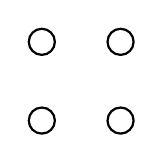
\begin{tikzpicture}[auto,
    specification/.style ={circle, draw, thick}]
   \node[specification] (A) at (0,0)  {};
   \node[specification] (B)  at (0,1)  {};
   \node[specification] (C)  at (1,1)  {};
   \node[specification] (D) at (1,0)  {};
 \end{tikzpicture}\\
 \vspace*{0.3cm}
 A
\end{minipage}\hfill 
  \begin{minipage}{0.24\linewidth}
    \centering
    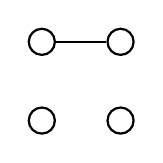
\begin{tikzpicture}[auto,
    specification/.style ={circle, draw, thick}]
   \node[specification] (A) at (0,0)  {};
   \node[specification] (B) at (0,1)  {};
   \node[specification] (C) at (1,1)  {};
   \node[specification] (D) at (1,0)  {};
   \draw[thick] (B) to  (C);
 \end{tikzpicture}\\
 \vspace*{0.3cm}
 B
\end{minipage}\hfill 
  \begin{minipage}{0.24\linewidth}
    \centering
    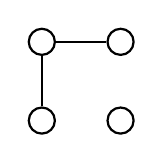
\begin{tikzpicture}[auto,
    specification/.style ={circle, draw, thick}]
   \node[specification] (A) at (0,0)  {};
   \node[specification] (B) at (0,1)  {};
   \node[specification] (C) at (1,1)  {};
   \node[specification] (D) at (1,0)  {};
   \draw[thick] (A) to  (B);
   \draw[thick] (B) to  (C);
 \end{tikzpicture}\\
 \vspace*{0.3cm}
 C
\end{minipage}\hfill 
  \begin{minipage}{0.24\linewidth}
    \centering
    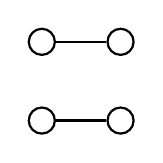
\begin{tikzpicture}[auto,
    specification/.style ={circle, draw, thick}]
   \node[specification] (A)  at (0,0)  {};
   \node[specification] (B)  at (0,1)  {};
   \node[specification] (C)  at (1,1)  {};
   \node[specification] (D) at (1,0)  {};
   \draw[thick] (B) to  (C);
   \draw[thick] (D) to  (A);
 \end{tikzpicture}\\
 \vspace*{0.3cm}
 D
\end{minipage}\hfill

\vspace*{0.5cm}
  \begin{minipage}{0.24\linewidth}
    \centering
    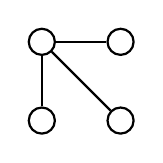
\begin{tikzpicture}[auto,
    specification/.style ={circle, draw, thick}]
   \node[specification] (A) at (0,0)  {};
   \node[specification] (B)  at (0,1)  {};
   \node[specification] (C)  at (1,1)  {};
   \node[specification] (D) at (1,0)  {};
   \draw[thick] (A) to (B);
   \draw[thick] (B) to (C);
      \draw[thick] (B) to (D);
 \end{tikzpicture}\\
 \vspace*{0.3cm}
 E
\end{minipage}\hfill
  \begin{minipage}{0.24\linewidth}
    \centering
    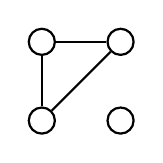
\begin{tikzpicture}[auto,
    specification/.style ={circle, draw, thick}]
   \node[specification] (A) at (0,0)  {};
   \node[specification] (B) at (0,1)  {};
   \node[specification] (C) at (1,1)  {};
   \node[specification] (D) at (1,0)  {};
   \draw[thick] (A) to  (B);
   \draw[thick] (B) to (C);
      \draw[thick] (C) to (A);
 \end{tikzpicture}\\
 \vspace*{0.3cm}
 F
\end{minipage}\hfill
  \begin{minipage}{0.24\linewidth}
    \centering
    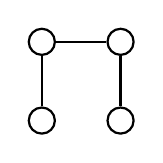
\begin{tikzpicture}[auto,
    specification/.style ={circle, draw, thick}]
   \node[specification] (A) at (0,0)  {};
   \node[specification] (B) at (0,1)  {};
   \node[specification] (C) at (1,1)  {};
   \node[specification] (D) at (1,0)  {};
   \draw[thick] (A) to  (B);
   \draw[thick] (B) to  (C);
      \draw[thick] (C) to (D);
 \end{tikzpicture}\\
 \vspace*{0.3cm}
 G
\end{minipage}\hfill 
  \begin{minipage}{0.24\linewidth}
    \centering
    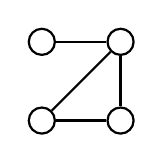
\begin{tikzpicture}[auto,
    specification/.style ={circle, draw, thick}]
   \node[specification] (A)  at (0,0)  {};
   \node[specification] (B)  at (0,1)  {};
   \node[specification] (C)  at (1,1)  {};
   \node[specification] (D) at (1,0)  {};
   \draw[thick] (A) to  (C);
   \draw[thick] (C) to  (D);
   \draw[thick] (D) to (A);
   \draw[thick] (C) to (B);
 \end{tikzpicture}\\
 \vspace*{0.3cm}
 H
\end{minipage}\hfill 

\vspace*{0.5cm}
\flushleft
  \begin{minipage}{0.24\linewidth}
    \centering
    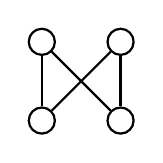
\begin{tikzpicture}[auto,
    specification/.style ={circle, draw, thick}]
   \node[specification] (A) at (0,0)  {};
   \node[specification] (B)  at (0,1)  {};
   \node[specification] (C)  at (1,1)  {};
   \node[specification] (D) at (1,0)  {};
   \draw[thick] (A) to (B);
   \draw[thick] (B) to (D);
   \draw[thick] (D) to (C);
      \draw[thick] (C) to (A);
 \end{tikzpicture}\\
 \vspace*{0.3cm}
 I
\end{minipage}
  \begin{minipage}{0.24\linewidth}
    \centering
    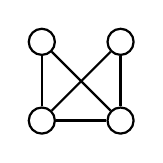
\begin{tikzpicture}[auto,
    specification/.style ={circle, draw, thick}]
   \node[specification] (A) at (0,0)  {};
   \node[specification] (B) at (0,1)  {};
   \node[specification] (C) at (1,1)  {};
   \node[specification] (D) at (1,0)  {};
   \draw[thick] (A) to  (B);
      \draw[thick] (C) to (D);
   \draw[thick] (D) to (A);
   \draw[thick] (A) to (C);
   \draw[thick] (B) to (D);
 \end{tikzpicture}\\
 \vspace*{0.3cm}
 J
\end{minipage} 
  \begin{minipage}{0.24\linewidth}
    \centering
    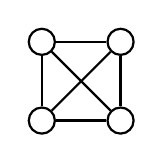
\begin{tikzpicture}[auto,
    specification/.style ={circle, draw, thick}]
   \node[specification] (A) at (0,0)  {};
   \node[specification] (B) at (0,1)  {};
   \node[specification] (C) at (1,1)  {};
   \node[specification] (D) at (1,0)  {};
   \draw[thick] (A) to  (B);
   \draw[thick] (B) to  (C);
      \draw[thick] (C) to (D);
   \draw[thick] (D) to (A);
   \draw[thick] (A) to (C);
   \draw[thick] (B) to (D);
 \end{tikzpicture}\\
 \vspace*{0.3cm}
 K
\end{minipage}

  \begin{Def}
    一个没有圈的无向图称为无向森林,简称{\bfseries森林}。
  \end{Def}
    在下列具有$4$个顶点的互相不同构的所有无向图中,有几个为森林?

    \vspace{0.3cm}
  \centering
  \begin{minipage}{0.24\linewidth}
    \centering
    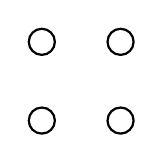
\begin{tikzpicture}[auto,
    specification/.style ={circle, draw, thick}]
   \node[specification] (A) at (0,0)  {};
   \node[specification] (B)  at (0,1)  {};
   \node[specification] (C)  at (1,1)  {};
   \node[specification] (D) at (1,0)  {};
 \end{tikzpicture}\\
 \vspace*{0.3cm}
 A
\end{minipage}\hfill 
  \begin{minipage}{0.24\linewidth}
    \centering
    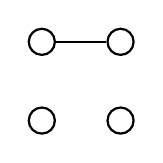
\begin{tikzpicture}[auto,
    specification/.style ={circle, draw, thick}]
   \node[specification] (A) at (0,0)  {};
   \node[specification] (B) at (0,1)  {};
   \node[specification] (C) at (1,1)  {};
   \node[specification] (D) at (1,0)  {};
   \draw[thick] (B) to  (C);
 \end{tikzpicture}\\
 \vspace*{0.3cm}
 B
\end{minipage}\hfill 
  \begin{minipage}{0.24\linewidth}
    \centering
    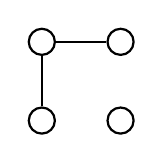
\begin{tikzpicture}[auto,
    specification/.style ={circle, draw, thick}]
   \node[specification] (A) at (0,0)  {};
   \node[specification] (B) at (0,1)  {};
   \node[specification] (C) at (1,1)  {};
   \node[specification] (D) at (1,0)  {};
   \draw[thick] (A) to  (B);
   \draw[thick] (B) to  (C);
 \end{tikzpicture}\\
 \vspace*{0.3cm}
 C
\end{minipage}\hfill 
  \begin{minipage}{0.24\linewidth}
    \centering
    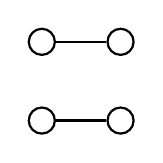
\begin{tikzpicture}[auto,
    specification/.style ={circle, draw, thick}]
   \node[specification] (A)  at (0,0)  {};
   \node[specification] (B)  at (0,1)  {};
   \node[specification] (C)  at (1,1)  {};
   \node[specification] (D) at (1,0)  {};
   \draw[thick] (B) to  (C);
   \draw[thick] (D) to  (A);
 \end{tikzpicture}\\
 \vspace*{0.3cm}
 D
\end{minipage}\hfill

\vspace*{0.5cm}
  \begin{minipage}{0.24\linewidth}
    \centering
    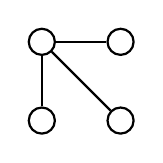
\begin{tikzpicture}[auto,
    specification/.style ={circle, draw, thick}]
   \node[specification] (A) at (0,0)  {};
   \node[specification] (B)  at (0,1)  {};
   \node[specification] (C)  at (1,1)  {};
   \node[specification] (D) at (1,0)  {};
   \draw[thick] (A) to (B);
   \draw[thick] (B) to (C);
      \draw[thick] (B) to (D);
 \end{tikzpicture}\\
 \vspace*{0.3cm}
 E
\end{minipage}\hfill
  \begin{minipage}{0.24\linewidth}
    \centering
    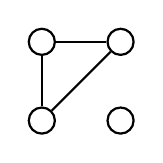
\begin{tikzpicture}[auto,
    specification/.style ={circle, draw, thick}]
   \node[specification] (A) at (0,0)  {};
   \node[specification] (B) at (0,1)  {};
   \node[specification] (C) at (1,1)  {};
   \node[specification] (D) at (1,0)  {};
   \draw[thick] (A) to  (B);
   \draw[thick] (B) to (C);
      \draw[thick] (C) to (A);
 \end{tikzpicture}\\
 \vspace*{0.3cm}
 F
\end{minipage}\hfill
  \begin{minipage}{0.24\linewidth}
    \centering
    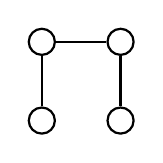
\begin{tikzpicture}[auto,
    specification/.style ={circle, draw, thick}]
   \node[specification] (A) at (0,0)  {};
   \node[specification] (B) at (0,1)  {};
   \node[specification] (C) at (1,1)  {};
   \node[specification] (D) at (1,0)  {};
   \draw[thick] (A) to  (B);
   \draw[thick] (B) to  (C);
      \draw[thick] (C) to (D);
 \end{tikzpicture}\\
 \vspace*{0.3cm}
 G
\end{minipage}\hfill 
  \begin{minipage}{0.24\linewidth}
    \centering
    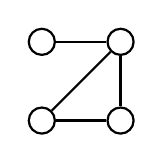
\begin{tikzpicture}[auto,
    specification/.style ={circle, draw, thick}]
   \node[specification] (A)  at (0,0)  {};
   \node[specification] (B)  at (0,1)  {};
   \node[specification] (C)  at (1,1)  {};
   \node[specification] (D) at (1,0)  {};
   \draw[thick] (A) to  (C);
   \draw[thick] (C) to  (D);
   \draw[thick] (D) to (A);
   \draw[thick] (C) to (B);
 \end{tikzpicture}\\
 \vspace*{0.3cm}
 H
\end{minipage}\hfill 

\vspace*{0.5cm}
\flushleft
  \begin{minipage}{0.24\linewidth}
    \centering
    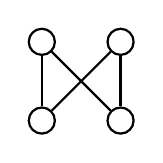
\begin{tikzpicture}[auto,
    specification/.style ={circle, draw, thick}]
   \node[specification] (A) at (0,0)  {};
   \node[specification] (B)  at (0,1)  {};
   \node[specification] (C)  at (1,1)  {};
   \node[specification] (D) at (1,0)  {};
   \draw[thick] (A) to (B);
   \draw[thick] (B) to (D);
   \draw[thick] (D) to (C);
      \draw[thick] (C) to (A);
 \end{tikzpicture}\\
 \vspace*{0.3cm}
 I
\end{minipage}
  \begin{minipage}{0.24\linewidth}
    \centering
    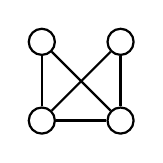
\begin{tikzpicture}[auto,
    specification/.style ={circle, draw, thick}]
   \node[specification] (A) at (0,0)  {};
   \node[specification] (B) at (0,1)  {};
   \node[specification] (C) at (1,1)  {};
   \node[specification] (D) at (1,0)  {};
   \draw[thick] (A) to  (B);
      \draw[thick] (C) to (D);
   \draw[thick] (D) to (A);
   \draw[thick] (A) to (C);
   \draw[thick] (B) to (D);
 \end{tikzpicture}\\
 \vspace*{0.3cm}
 J
\end{minipage} 
  \begin{minipage}{0.24\linewidth}
    \centering
    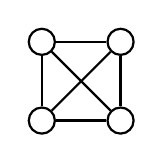
\begin{tikzpicture}[auto,
    specification/.style ={circle, draw, thick}]
   \node[specification] (A) at (0,0)  {};
   \node[specification] (B) at (0,1)  {};
   \node[specification] (C) at (1,1)  {};
   \node[specification] (D) at (1,0)  {};
   \draw[thick] (A) to  (B);
   \draw[thick] (B) to  (C);
      \draw[thick] (C) to (D);
   \draw[thick] (D) to (A);
   \draw[thick] (A) to (C);
   \draw[thick] (B) to (D);
 \end{tikzpicture}\\
 \vspace*{0.3cm}
 K
\end{minipage}

\clearpage
    \begin{Def}
    设$G=(V,E)$为一个图,$G$的一个生成子图$T=(V,F)$如果是树,则称$T$为$G$的{\bfseries 生成树}。
  \end{Def}
      在下列具有$4$个顶点的互相不同构的所有无向图中,有几个无向图有一棵生成树与图$E$同构?

    \vspace{0.3cm}
  \centering
  \begin{minipage}{0.24\linewidth}
    \centering
    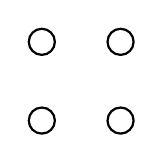
\begin{tikzpicture}[auto,
    specification/.style ={circle, draw, thick}]
   \node[specification] (A) at (0,0)  {};
   \node[specification] (B)  at (0,1)  {};
   \node[specification] (C)  at (1,1)  {};
   \node[specification] (D) at (1,0)  {};
 \end{tikzpicture}\\
 \vspace*{0.3cm}
 A
\end{minipage}\hfill 
  \begin{minipage}{0.24\linewidth}
    \centering
    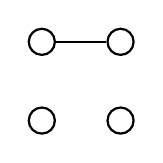
\begin{tikzpicture}[auto,
    specification/.style ={circle, draw, thick}]
   \node[specification] (A) at (0,0)  {};
   \node[specification] (B) at (0,1)  {};
   \node[specification] (C) at (1,1)  {};
   \node[specification] (D) at (1,0)  {};
   \draw[thick] (B) to  (C);
 \end{tikzpicture}\\
 \vspace*{0.3cm}
 B
\end{minipage}\hfill 
  \begin{minipage}{0.24\linewidth}
    \centering
    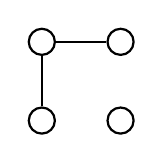
\begin{tikzpicture}[auto,
    specification/.style ={circle, draw, thick}]
   \node[specification] (A) at (0,0)  {};
   \node[specification] (B) at (0,1)  {};
   \node[specification] (C) at (1,1)  {};
   \node[specification] (D) at (1,0)  {};
   \draw[thick] (A) to  (B);
   \draw[thick] (B) to  (C);
 \end{tikzpicture}\\
 \vspace*{0.3cm}
 C
\end{minipage}\hfill 
  \begin{minipage}{0.24\linewidth}
    \centering
    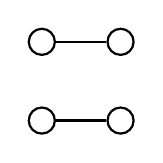
\begin{tikzpicture}[auto,
    specification/.style ={circle, draw, thick}]
   \node[specification] (A)  at (0,0)  {};
   \node[specification] (B)  at (0,1)  {};
   \node[specification] (C)  at (1,1)  {};
   \node[specification] (D) at (1,0)  {};
   \draw[thick] (B) to  (C);
   \draw[thick] (D) to  (A);
 \end{tikzpicture}\\
 \vspace*{0.3cm}
 D
\end{minipage}\hfill

\vspace*{0.5cm}
  \begin{minipage}{0.24\linewidth}
    \centering
    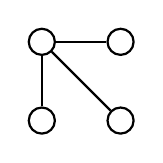
\begin{tikzpicture}[auto,
    specification/.style ={circle, draw, thick}]
   \node[specification] (A) at (0,0)  {};
   \node[specification] (B)  at (0,1)  {};
   \node[specification] (C)  at (1,1)  {};
   \node[specification] (D) at (1,0)  {};
   \draw[thick] (A) to (B);
   \draw[thick] (B) to (C);
      \draw[thick] (B) to (D);
 \end{tikzpicture}\\
 \vspace*{0.3cm}
 E
\end{minipage}\hfill
  \begin{minipage}{0.24\linewidth}
    \centering
    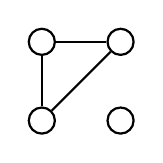
\begin{tikzpicture}[auto,
    specification/.style ={circle, draw, thick}]
   \node[specification] (A) at (0,0)  {};
   \node[specification] (B) at (0,1)  {};
   \node[specification] (C) at (1,1)  {};
   \node[specification] (D) at (1,0)  {};
   \draw[thick] (A) to  (B);
   \draw[thick] (B) to (C);
      \draw[thick] (C) to (A);
 \end{tikzpicture}\\
 \vspace*{0.3cm}
 F
\end{minipage}\hfill
  \begin{minipage}{0.24\linewidth}
    \centering
    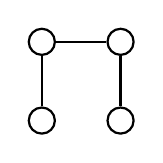
\begin{tikzpicture}[auto,
    specification/.style ={circle, draw, thick}]
   \node[specification] (A) at (0,0)  {};
   \node[specification] (B) at (0,1)  {};
   \node[specification] (C) at (1,1)  {};
   \node[specification] (D) at (1,0)  {};
   \draw[thick] (A) to  (B);
   \draw[thick] (B) to  (C);
      \draw[thick] (C) to (D);
 \end{tikzpicture}\\
 \vspace*{0.3cm}
 G
\end{minipage}\hfill 
  \begin{minipage}{0.24\linewidth}
    \centering
    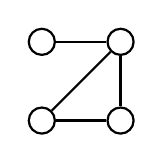
\begin{tikzpicture}[auto,
    specification/.style ={circle, draw, thick}]
   \node[specification] (A)  at (0,0)  {};
   \node[specification] (B)  at (0,1)  {};
   \node[specification] (C)  at (1,1)  {};
   \node[specification] (D) at (1,0)  {};
   \draw[thick] (A) to  (C);
   \draw[thick] (C) to  (D);
   \draw[thick] (D) to (A);
   \draw[thick] (C) to (B);
 \end{tikzpicture}\\
 \vspace*{0.3cm}
 H
\end{minipage}\hfill 

\vspace*{0.5cm}
\flushleft
  \begin{minipage}{0.24\linewidth}
    \centering
    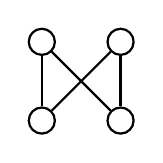
\begin{tikzpicture}[auto,
    specification/.style ={circle, draw, thick}]
   \node[specification] (A) at (0,0)  {};
   \node[specification] (B)  at (0,1)  {};
   \node[specification] (C)  at (1,1)  {};
   \node[specification] (D) at (1,0)  {};
   \draw[thick] (A) to (B);
   \draw[thick] (B) to (D);
   \draw[thick] (D) to (C);
      \draw[thick] (C) to (A);
 \end{tikzpicture}\\
 \vspace*{0.3cm}
 I
\end{minipage}
  \begin{minipage}{0.24\linewidth}
    \centering
    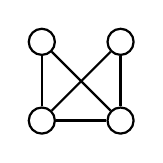
\begin{tikzpicture}[auto,
    specification/.style ={circle, draw, thick}]
   \node[specification] (A) at (0,0)  {};
   \node[specification] (B) at (0,1)  {};
   \node[specification] (C) at (1,1)  {};
   \node[specification] (D) at (1,0)  {};
   \draw[thick] (A) to  (B);
      \draw[thick] (C) to (D);
   \draw[thick] (D) to (A);
   \draw[thick] (A) to (C);
   \draw[thick] (B) to (D);
 \end{tikzpicture}\\
 \vspace*{0.3cm}
 J
\end{minipage} 
  \begin{minipage}{0.24\linewidth}
    \centering
    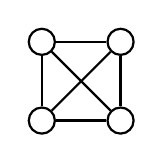
\begin{tikzpicture}[auto,
    specification/.style ={circle, draw, thick}]
   \node[specification] (A) at (0,0)  {};
   \node[specification] (B) at (0,1)  {};
   \node[specification] (C) at (1,1)  {};
   \node[specification] (D) at (1,0)  {};
   \draw[thick] (A) to  (B);
   \draw[thick] (B) to  (C);
      \draw[thick] (C) to (D);
   \draw[thick] (D) to (A);
   \draw[thick] (A) to (C);
   \draw[thick] (B) to (D);
 \end{tikzpicture}\\
 \vspace*{0.3cm}
 K
\end{minipage}
    \begin{Def}
    设$G=(V,E)$为一个图,$G$的一个生成子图$T=(V,F)$如果是树,则称$T$为$G$的{\bfseries 生成树}。
  \end{Def}
      在下列具有$4$个顶点的互相不同构的所有无向图中,有几个无向图有一棵生成树与图$G$同构?

    \vspace{0.3cm}
  \centering
  \begin{minipage}{0.24\linewidth}
    \centering
    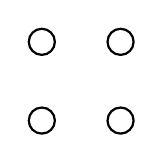
\begin{tikzpicture}[auto,
    specification/.style ={circle, draw, thick}]
   \node[specification] (A) at (0,0)  {};
   \node[specification] (B)  at (0,1)  {};
   \node[specification] (C)  at (1,1)  {};
   \node[specification] (D) at (1,0)  {};
 \end{tikzpicture}\\
 \vspace*{0.3cm}
 A
\end{minipage}\hfill 
  \begin{minipage}{0.24\linewidth}
    \centering
    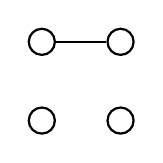
\begin{tikzpicture}[auto,
    specification/.style ={circle, draw, thick}]
   \node[specification] (A) at (0,0)  {};
   \node[specification] (B) at (0,1)  {};
   \node[specification] (C) at (1,1)  {};
   \node[specification] (D) at (1,0)  {};
   \draw[thick] (B) to  (C);
 \end{tikzpicture}\\
 \vspace*{0.3cm}
 B
\end{minipage}\hfill 
  \begin{minipage}{0.24\linewidth}
    \centering
    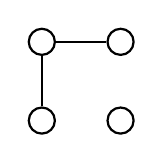
\begin{tikzpicture}[auto,
    specification/.style ={circle, draw, thick}]
   \node[specification] (A) at (0,0)  {};
   \node[specification] (B) at (0,1)  {};
   \node[specification] (C) at (1,1)  {};
   \node[specification] (D) at (1,0)  {};
   \draw[thick] (A) to  (B);
   \draw[thick] (B) to  (C);
 \end{tikzpicture}\\
 \vspace*{0.3cm}
 C
\end{minipage}\hfill 
  \begin{minipage}{0.24\linewidth}
    \centering
    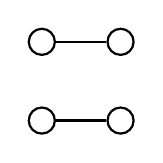
\begin{tikzpicture}[auto,
    specification/.style ={circle, draw, thick}]
   \node[specification] (A)  at (0,0)  {};
   \node[specification] (B)  at (0,1)  {};
   \node[specification] (C)  at (1,1)  {};
   \node[specification] (D) at (1,0)  {};
   \draw[thick] (B) to  (C);
   \draw[thick] (D) to  (A);
 \end{tikzpicture}\\
 \vspace*{0.3cm}
 D
\end{minipage}\hfill

\vspace*{0.5cm}
  \begin{minipage}{0.24\linewidth}
    \centering
    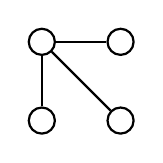
\begin{tikzpicture}[auto,
    specification/.style ={circle, draw, thick}]
   \node[specification] (A) at (0,0)  {};
   \node[specification] (B)  at (0,1)  {};
   \node[specification] (C)  at (1,1)  {};
   \node[specification] (D) at (1,0)  {};
   \draw[thick] (A) to (B);
   \draw[thick] (B) to (C);
      \draw[thick] (B) to (D);
 \end{tikzpicture}\\
 \vspace*{0.3cm}
 E
\end{minipage}\hfill
  \begin{minipage}{0.24\linewidth}
    \centering
    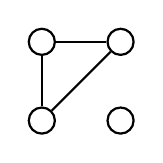
\begin{tikzpicture}[auto,
    specification/.style ={circle, draw, thick}]
   \node[specification] (A) at (0,0)  {};
   \node[specification] (B) at (0,1)  {};
   \node[specification] (C) at (1,1)  {};
   \node[specification] (D) at (1,0)  {};
   \draw[thick] (A) to  (B);
   \draw[thick] (B) to (C);
      \draw[thick] (C) to (A);
 \end{tikzpicture}\\
 \vspace*{0.3cm}
 F
\end{minipage}\hfill
  \begin{minipage}{0.24\linewidth}
    \centering
    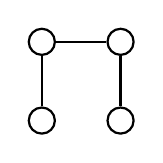
\begin{tikzpicture}[auto,
    specification/.style ={circle, draw, thick}]
   \node[specification] (A) at (0,0)  {};
   \node[specification] (B) at (0,1)  {};
   \node[specification] (C) at (1,1)  {};
   \node[specification] (D) at (1,0)  {};
   \draw[thick] (A) to  (B);
   \draw[thick] (B) to  (C);
      \draw[thick] (C) to (D);
 \end{tikzpicture}\\
 \vspace*{0.3cm}
 G
\end{minipage}\hfill 
  \begin{minipage}{0.24\linewidth}
    \centering
    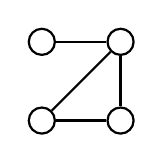
\begin{tikzpicture}[auto,
    specification/.style ={circle, draw, thick}]
   \node[specification] (A)  at (0,0)  {};
   \node[specification] (B)  at (0,1)  {};
   \node[specification] (C)  at (1,1)  {};
   \node[specification] (D) at (1,0)  {};
   \draw[thick] (A) to  (C);
   \draw[thick] (C) to  (D);
   \draw[thick] (D) to (A);
   \draw[thick] (C) to (B);
 \end{tikzpicture}\\
 \vspace*{0.3cm}
 H
\end{minipage}\hfill 

\vspace*{0.5cm}
\flushleft
  \begin{minipage}{0.24\linewidth}
    \centering
    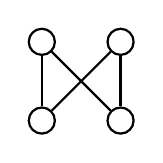
\begin{tikzpicture}[auto,
    specification/.style ={circle, draw, thick}]
   \node[specification] (A) at (0,0)  {};
   \node[specification] (B)  at (0,1)  {};
   \node[specification] (C)  at (1,1)  {};
   \node[specification] (D) at (1,0)  {};
   \draw[thick] (A) to (B);
   \draw[thick] (B) to (D);
   \draw[thick] (D) to (C);
      \draw[thick] (C) to (A);
 \end{tikzpicture}\\
 \vspace*{0.3cm}
 I
\end{minipage}
  \begin{minipage}{0.24\linewidth}
    \centering
    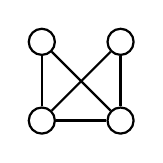
\begin{tikzpicture}[auto,
    specification/.style ={circle, draw, thick}]
   \node[specification] (A) at (0,0)  {};
   \node[specification] (B) at (0,1)  {};
   \node[specification] (C) at (1,1)  {};
   \node[specification] (D) at (1,0)  {};
   \draw[thick] (A) to  (B);
      \draw[thick] (C) to (D);
   \draw[thick] (D) to (A);
   \draw[thick] (A) to (C);
   \draw[thick] (B) to (D);
 \end{tikzpicture}\\
 \vspace*{0.3cm}
 J
\end{minipage} 
  \begin{minipage}{0.24\linewidth}
    \centering
    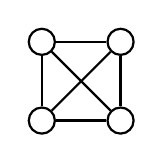
\begin{tikzpicture}[auto,
    specification/.style ={circle, draw, thick}]
   \node[specification] (A) at (0,0)  {};
   \node[specification] (B) at (0,1)  {};
   \node[specification] (C) at (1,1)  {};
   \node[specification] (D) at (1,0)  {};
   \draw[thick] (A) to  (B);
   \draw[thick] (B) to  (C);
      \draw[thick] (C) to (D);
   \draw[thick] (D) to (A);
   \draw[thick] (A) to (C);
   \draw[thick] (B) to (D);
 \end{tikzpicture}\\
 \vspace*{0.3cm}
 K
\end{minipage}

  \begin{Def}
    设$v$为图$G$的一个顶点,如果$G-v$的支数大于$G$的支数,则称顶点$v$为图$G$的一个{\bfseries 割点}。
  \end{Def}
      在下列具有$4$个顶点的互相不同构的所有无向图中,有几个图有且仅有两个割点?

    \vspace{0.3cm}
  \centering
  \begin{minipage}{0.24\linewidth}
    \centering
    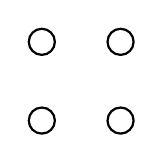
\begin{tikzpicture}[auto,
    specification/.style ={circle, draw, thick}]
   \node[specification] (A) at (0,0)  {};
   \node[specification] (B)  at (0,1)  {};
   \node[specification] (C)  at (1,1)  {};
   \node[specification] (D) at (1,0)  {};
 \end{tikzpicture}\\
 \vspace*{0.3cm}
 A
\end{minipage}\hfill 
  \begin{minipage}{0.24\linewidth}
    \centering
    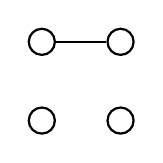
\begin{tikzpicture}[auto,
    specification/.style ={circle, draw, thick}]
   \node[specification] (A) at (0,0)  {};
   \node[specification] (B) at (0,1)  {};
   \node[specification] (C) at (1,1)  {};
   \node[specification] (D) at (1,0)  {};
   \draw[thick] (B) to  (C);
 \end{tikzpicture}\\
 \vspace*{0.3cm}
 B
\end{minipage}\hfill 
  \begin{minipage}{0.24\linewidth}
    \centering
    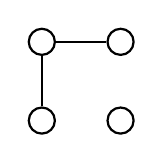
\begin{tikzpicture}[auto,
    specification/.style ={circle, draw, thick}]
   \node[specification] (A) at (0,0)  {};
   \node[specification] (B) at (0,1)  {};
   \node[specification] (C) at (1,1)  {};
   \node[specification] (D) at (1,0)  {};
   \draw[thick] (A) to  (B);
   \draw[thick] (B) to  (C);
 \end{tikzpicture}\\
 \vspace*{0.3cm}
 C
\end{minipage}\hfill 
  \begin{minipage}{0.24\linewidth}
    \centering
    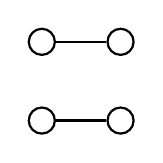
\begin{tikzpicture}[auto,
    specification/.style ={circle, draw, thick}]
   \node[specification] (A)  at (0,0)  {};
   \node[specification] (B)  at (0,1)  {};
   \node[specification] (C)  at (1,1)  {};
   \node[specification] (D) at (1,0)  {};
   \draw[thick] (B) to  (C);
   \draw[thick] (D) to  (A);
 \end{tikzpicture}\\
 \vspace*{0.3cm}
 D
\end{minipage}\hfill

\vspace*{0.5cm}
  \begin{minipage}{0.24\linewidth}
    \centering
    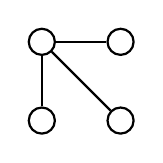
\begin{tikzpicture}[auto,
    specification/.style ={circle, draw, thick}]
   \node[specification] (A) at (0,0)  {};
   \node[specification] (B)  at (0,1)  {};
   \node[specification] (C)  at (1,1)  {};
   \node[specification] (D) at (1,0)  {};
   \draw[thick] (A) to (B);
   \draw[thick] (B) to (C);
      \draw[thick] (B) to (D);
 \end{tikzpicture}\\
 \vspace*{0.3cm}
 E
\end{minipage}\hfill
  \begin{minipage}{0.24\linewidth}
    \centering
    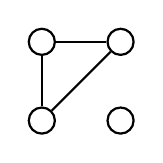
\begin{tikzpicture}[auto,
    specification/.style ={circle, draw, thick}]
   \node[specification] (A) at (0,0)  {};
   \node[specification] (B) at (0,1)  {};
   \node[specification] (C) at (1,1)  {};
   \node[specification] (D) at (1,0)  {};
   \draw[thick] (A) to  (B);
   \draw[thick] (B) to (C);
      \draw[thick] (C) to (A);
 \end{tikzpicture}\\
 \vspace*{0.3cm}
 F
\end{minipage}\hfill
  \begin{minipage}{0.24\linewidth}
    \centering
    \begin{tikzpicture}[auto,
    specification/.style ={circle, draw, thick}]
   \node[specification] (A) at (0,0)  {};
   \node[specification] (B) at (0,1)  {};
   \node[specification] (C) at (1,1)  {};
   \node[specification] (D) at (1,0)  {};
   \draw[thick] (A) to  (B);
   \draw[thick] (B) to  (C);
      \draw[thick] (C) to (D);
 \end{tikzpicture}\\
 \vspace*{0.3cm}
 G
\end{minipage}\hfill 
  \begin{minipage}{0.24\linewidth}
    \centering
    \begin{tikzpicture}[auto,
    specification/.style ={circle, draw, thick}]
   \node[specification] (A)  at (0,0)  {};
   \node[specification] (B)  at (0,1)  {};
   \node[specification] (C)  at (1,1)  {};
   \node[specification] (D) at (1,0)  {};
   \draw[thick] (A) to  (C);
   \draw[thick] (C) to  (D);
   \draw[thick] (D) to (A);
   \draw[thick] (C) to (B);
 \end{tikzpicture}\\
 \vspace*{0.3cm}
 H
\end{minipage}\hfill 

\vspace*{0.5cm}
\flushleft
  \begin{minipage}{0.24\linewidth}
    \centering
    \begin{tikzpicture}[auto,
    specification/.style ={circle, draw, thick}]
   \node[specification] (A) at (0,0)  {};
   \node[specification] (B)  at (0,1)  {};
   \node[specification] (C)  at (1,1)  {};
   \node[specification] (D) at (1,0)  {};
   \draw[thick] (A) to (B);
   \draw[thick] (B) to (D);
   \draw[thick] (D) to (C);
      \draw[thick] (C) to (A);
 \end{tikzpicture}\\
 \vspace*{0.3cm}
 I
\end{minipage}
  \begin{minipage}{0.24\linewidth}
    \centering
    \begin{tikzpicture}[auto,
    specification/.style ={circle, draw, thick}]
   \node[specification] (A) at (0,0)  {};
   \node[specification] (B) at (0,1)  {};
   \node[specification] (C) at (1,1)  {};
   \node[specification] (D) at (1,0)  {};
   \draw[thick] (A) to  (B);
      \draw[thick] (C) to (D);
   \draw[thick] (D) to (A);
   \draw[thick] (A) to (C);
   \draw[thick] (B) to (D);
 \end{tikzpicture}\\
 \vspace*{0.3cm}
 J
\end{minipage} 
  \begin{minipage}{0.24\linewidth}
    \centering
    \begin{tikzpicture}[auto,
    specification/.style ={circle, draw, thick}]
   \node[specification] (A) at (0,0)  {};
   \node[specification] (B) at (0,1)  {};
   \node[specification] (C) at (1,1)  {};
   \node[specification] (D) at (1,0)  {};
   \draw[thick] (A) to  (B);
   \draw[thick] (B) to  (C);
      \draw[thick] (C) to (D);
   \draw[thick] (D) to (A);
   \draw[thick] (A) to (C);
   \draw[thick] (B) to (D);
 \end{tikzpicture}\\
 \vspace*{0.3cm}
 K
\end{minipage}

  \begin{Def}
   图$G$的一条边$x$称为$G$的一座{\bfseries 桥},如果$G-x$的支数大于$G$的支数。
 \end{Def}
     在下列具有$4$个顶点的互相不同构的所有无向图中,有几个无向图有且仅有两条割边?

    \vspace{0.3cm}
  \centering
  \begin{minipage}{0.24\linewidth}
    \centering
    \begin{tikzpicture}[auto,
    specification/.style ={circle, draw, thick}]
   \node[specification] (A) at (0,0)  {};
   \node[specification] (B)  at (0,1)  {};
   \node[specification] (C)  at (1,1)  {};
   \node[specification] (D) at (1,0)  {};
 \end{tikzpicture}\\
 \vspace*{0.3cm}
 A
\end{minipage}\hfill 
  \begin{minipage}{0.24\linewidth}
    \centering
    \begin{tikzpicture}[auto,
    specification/.style ={circle, draw, thick}]
   \node[specification] (A) at (0,0)  {};
   \node[specification] (B) at (0,1)  {};
   \node[specification] (C) at (1,1)  {};
   \node[specification] (D) at (1,0)  {};
   \draw[thick] (B) to  (C);
 \end{tikzpicture}\\
 \vspace*{0.3cm}
 B
\end{minipage}\hfill 
  \begin{minipage}{0.24\linewidth}
    \centering
    \begin{tikzpicture}[auto,
    specification/.style ={circle, draw, thick}]
   \node[specification] (A) at (0,0)  {};
   \node[specification] (B) at (0,1)  {};
   \node[specification] (C) at (1,1)  {};
   \node[specification] (D) at (1,0)  {};
   \draw[thick] (A) to  (B);
   \draw[thick] (B) to  (C);
 \end{tikzpicture}\\
 \vspace*{0.3cm}
 C
\end{minipage}\hfill 
  \begin{minipage}{0.24\linewidth}
    \centering
    \begin{tikzpicture}[auto,
    specification/.style ={circle, draw, thick}]
   \node[specification] (A)  at (0,0)  {};
   \node[specification] (B)  at (0,1)  {};
   \node[specification] (C)  at (1,1)  {};
   \node[specification] (D) at (1,0)  {};
   \draw[thick] (B) to  (C);
   \draw[thick] (D) to  (A);
 \end{tikzpicture}\\
 \vspace*{0.3cm}
 D
\end{minipage}\hfill

\vspace*{0.5cm}
  \begin{minipage}{0.24\linewidth}
    \centering
    \begin{tikzpicture}[auto,
    specification/.style ={circle, draw, thick}]
   \node[specification] (A) at (0,0)  {};
   \node[specification] (B)  at (0,1)  {};
   \node[specification] (C)  at (1,1)  {};
   \node[specification] (D) at (1,0)  {};
   \draw[thick] (A) to (B);
   \draw[thick] (B) to (C);
      \draw[thick] (B) to (D);
 \end{tikzpicture}\\
 \vspace*{0.3cm}
 E
\end{minipage}\hfill
  \begin{minipage}{0.24\linewidth}
    \centering
    \begin{tikzpicture}[auto,
    specification/.style ={circle, draw, thick}]
   \node[specification] (A) at (0,0)  {};
   \node[specification] (B) at (0,1)  {};
   \node[specification] (C) at (1,1)  {};
   \node[specification] (D) at (1,0)  {};
   \draw[thick] (A) to  (B);
   \draw[thick] (B) to (C);
      \draw[thick] (C) to (A);
 \end{tikzpicture}\\
 \vspace*{0.3cm}
 F
\end{minipage}\hfill
  \begin{minipage}{0.24\linewidth}
    \centering
    \begin{tikzpicture}[auto,
    specification/.style ={circle, draw, thick}]
   \node[specification] (A) at (0,0)  {};
   \node[specification] (B) at (0,1)  {};
   \node[specification] (C) at (1,1)  {};
   \node[specification] (D) at (1,0)  {};
   \draw[thick] (A) to  (B);
   \draw[thick] (B) to  (C);
      \draw[thick] (C) to (D);
 \end{tikzpicture}\\
 \vspace*{0.3cm}
 G
\end{minipage}\hfill 
  \begin{minipage}{0.24\linewidth}
    \centering
    \begin{tikzpicture}[auto,
    specification/.style ={circle, draw, thick}]
   \node[specification] (A)  at (0,0)  {};
   \node[specification] (B)  at (0,1)  {};
   \node[specification] (C)  at (1,1)  {};
   \node[specification] (D) at (1,0)  {};
   \draw[thick] (A) to  (C);
   \draw[thick] (C) to  (D);
   \draw[thick] (D) to (A);
   \draw[thick] (C) to (B);
 \end{tikzpicture}\\
 \vspace*{0.3cm}
 H
\end{minipage}\hfill 

\vspace*{0.5cm}
\flushleft
  \begin{minipage}{0.24\linewidth}
    \centering
    \begin{tikzpicture}[auto,
    specification/.style ={circle, draw, thick}]
   \node[specification] (A) at (0,0)  {};
   \node[specification] (B)  at (0,1)  {};
   \node[specification] (C)  at (1,1)  {};
   \node[specification] (D) at (1,0)  {};
   \draw[thick] (A) to (B);
   \draw[thick] (B) to (D);
   \draw[thick] (D) to (C);
      \draw[thick] (C) to (A);
 \end{tikzpicture}\\
 \vspace*{0.3cm}
 I
\end{minipage}
  \begin{minipage}{0.24\linewidth}
    \centering
    \begin{tikzpicture}[auto,
    specification/.style ={circle, draw, thick}]
   \node[specification] (A) at (0,0)  {};
   \node[specification] (B) at (0,1)  {};
   \node[specification] (C) at (1,1)  {};
   \node[specification] (D) at (1,0)  {};
   \draw[thick] (A) to  (B);
      \draw[thick] (C) to (D);
   \draw[thick] (D) to (A);
   \draw[thick] (A) to (C);
   \draw[thick] (B) to (D);
 \end{tikzpicture}\\
 \vspace*{0.3cm}
 J
\end{minipage} 
  \begin{minipage}{0.24\linewidth}
    \centering
    \begin{tikzpicture}[auto,
    specification/.style ={circle, draw, thick}]
   \node[specification] (A) at (0,0)  {};
   \node[specification] (B) at (0,1)  {};
   \node[specification] (C) at (1,1)  {};
   \node[specification] (D) at (1,0)  {};
   \draw[thick] (A) to  (B);
   \draw[thick] (B) to  (C);
      \draw[thick] (C) to (D);
   \draw[thick] (D) to (A);
   \draw[thick] (A) to (C);
   \draw[thick] (B) to (D);
 \end{tikzpicture}\\
 \vspace*{0.3cm}
 K
\end{minipage}

  \begin{Def}
    设$G = (V,E)$为图,$S \subseteq E$。如果从$G$中去掉$S$中的所有边得到的图$G-S$的支数大于$G$的支数,而去掉$S$的任一真子集中的边得到的图的支数不大于$G$的支数,则称$S$为$G$的一个{\bfseries 割集}。
  \end{Def}
      在下列具有$4$个顶点的互相不同构的所有无向图中,图$H$有几个互不相同的割集?

    \vspace{0.3cm}
  \centering
  \begin{minipage}{0.24\linewidth}
    \centering
    \begin{tikzpicture}[auto,
    specification/.style ={circle, draw, thick}]
   \node[specification] (A) at (0,0)  {};
   \node[specification] (B)  at (0,1)  {};
   \node[specification] (C)  at (1,1)  {};
   \node[specification] (D) at (1,0)  {};
 \end{tikzpicture}\\
 \vspace*{0.3cm}
 A
\end{minipage}\hfill 
  \begin{minipage}{0.24\linewidth}
    \centering
    \begin{tikzpicture}[auto,
    specification/.style ={circle, draw, thick}]
   \node[specification] (A) at (0,0)  {};
   \node[specification] (B) at (0,1)  {};
   \node[specification] (C) at (1,1)  {};
   \node[specification] (D) at (1,0)  {};
   \draw[thick] (B) to  (C);
 \end{tikzpicture}\\
 \vspace*{0.3cm}
 B
\end{minipage}\hfill 
  \begin{minipage}{0.24\linewidth}
    \centering
    \begin{tikzpicture}[auto,
    specification/.style ={circle, draw, thick}]
   \node[specification] (A) at (0,0)  {};
   \node[specification] (B) at (0,1)  {};
   \node[specification] (C) at (1,1)  {};
   \node[specification] (D) at (1,0)  {};
   \draw[thick] (A) to  (B);
   \draw[thick] (B) to  (C);
 \end{tikzpicture}\\
 \vspace*{0.3cm}
 C
\end{minipage}\hfill 
  \begin{minipage}{0.24\linewidth}
    \centering
    \begin{tikzpicture}[auto,
    specification/.style ={circle, draw, thick}]
   \node[specification] (A)  at (0,0)  {};
   \node[specification] (B)  at (0,1)  {};
   \node[specification] (C)  at (1,1)  {};
   \node[specification] (D) at (1,0)  {};
   \draw[thick] (B) to  (C);
   \draw[thick] (D) to  (A);
 \end{tikzpicture}\\
 \vspace*{0.3cm}
 D
\end{minipage}\hfill

\vspace*{0.5cm}
  \begin{minipage}{0.24\linewidth}
    \centering
    \begin{tikzpicture}[auto,
    specification/.style ={circle, draw, thick}]
   \node[specification] (A) at (0,0)  {};
   \node[specification] (B)  at (0,1)  {};
   \node[specification] (C)  at (1,1)  {};
   \node[specification] (D) at (1,0)  {};
   \draw[thick] (A) to (B);
   \draw[thick] (B) to (C);
      \draw[thick] (B) to (D);
 \end{tikzpicture}\\
 \vspace*{0.3cm}
 E
\end{minipage}\hfill
  \begin{minipage}{0.24\linewidth}
    \centering
    \begin{tikzpicture}[auto,
    specification/.style ={circle, draw, thick}]
   \node[specification] (A) at (0,0)  {};
   \node[specification] (B) at (0,1)  {};
   \node[specification] (C) at (1,1)  {};
   \node[specification] (D) at (1,0)  {};
   \draw[thick] (A) to  (B);
   \draw[thick] (B) to (C);
      \draw[thick] (C) to (A);
 \end{tikzpicture}\\
 \vspace*{0.3cm}
 F
\end{minipage}\hfill
  \begin{minipage}{0.24\linewidth}
    \centering
    \begin{tikzpicture}[auto,
    specification/.style ={circle, draw, thick}]
   \node[specification] (A) at (0,0)  {};
   \node[specification] (B) at (0,1)  {};
   \node[specification] (C) at (1,1)  {};
   \node[specification] (D) at (1,0)  {};
   \draw[thick] (A) to  (B);
   \draw[thick] (B) to  (C);
      \draw[thick] (C) to (D);
 \end{tikzpicture}\\
 \vspace*{0.3cm}
 G
\end{minipage}\hfill 
  \begin{minipage}{0.24\linewidth}
    \centering
    \begin{tikzpicture}[auto,
    specification/.style ={circle, draw, thick}]
   \node[specification] (A)  at (0,0)  {};
   \node[specification] (B)  at (0,1)  {};
   \node[specification] (C)  at (1,1)  {};
   \node[specification] (D) at (1,0)  {};
   \draw[thick] (A) to  (C);
   \draw[thick] (C) to  (D);
   \draw[thick] (D) to (A);
   \draw[thick] (C) to (B);
 \end{tikzpicture}\\
 \vspace*{0.3cm}
 H
\end{minipage}\hfill 

\vspace*{0.5cm}
\flushleft
  \begin{minipage}{0.24\linewidth}
    \centering
    \begin{tikzpicture}[auto,
    specification/.style ={circle, draw, thick}]
   \node[specification] (A) at (0,0)  {};
   \node[specification] (B)  at (0,1)  {};
   \node[specification] (C)  at (1,1)  {};
   \node[specification] (D) at (1,0)  {};
   \draw[thick] (A) to (B);
   \draw[thick] (B) to (D);
   \draw[thick] (D) to (C);
      \draw[thick] (C) to (A);
 \end{tikzpicture}\\
 \vspace*{0.3cm}
 I
\end{minipage}
  \begin{minipage}{0.24\linewidth}
    \centering
    \begin{tikzpicture}[auto,
    specification/.style ={circle, draw, thick}]
   \node[specification] (A) at (0,0)  {};
   \node[specification] (B) at (0,1)  {};
   \node[specification] (C) at (1,1)  {};
   \node[specification] (D) at (1,0)  {};
   \draw[thick] (A) to  (B);
      \draw[thick] (C) to (D);
   \draw[thick] (D) to (A);
   \draw[thick] (A) to (C);
   \draw[thick] (B) to (D);
 \end{tikzpicture}\\
 \vspace*{0.3cm}
 J
\end{minipage} 
  \begin{minipage}{0.24\linewidth}
    \centering
    \begin{tikzpicture}[auto,
    specification/.style ={circle, draw, thick}]
   \node[specification] (A) at (0,0)  {};
   \node[specification] (B) at (0,1)  {};
   \node[specification] (C) at (1,1)  {};
   \node[specification] (D) at (1,0)  {};
   \draw[thick] (A) to  (B);
   \draw[thick] (B) to  (C);
      \draw[thick] (C) to (D);
   \draw[thick] (D) to (A);
   \draw[thick] (A) to (C);
   \draw[thick] (B) to (D);
 \end{tikzpicture}\\
 \vspace*{0.3cm}
 K
\end{minipage}


  \begin{Def}
    图$G$的{\bfseries 顶点连通度}是指为了产生一个不连通图或平凡图所需要从$G$中去掉的最少顶点数目, 记为$\kappa (G)$。
  \end{Def}

      在下列具有$4$个顶点的互相不同构的所有无向图中,有几个顶点连通度为$2$?

    \vspace{0.3cm}
  \centering
  \begin{minipage}{0.24\linewidth}
    \centering
    \begin{tikzpicture}[auto,
    specification/.style ={circle, draw, thick}]
   \node[specification] (A) at (0,0)  {};
   \node[specification] (B)  at (0,1)  {};
   \node[specification] (C)  at (1,1)  {};
   \node[specification] (D) at (1,0)  {};
 \end{tikzpicture}\\
 \vspace*{0.3cm}
 A
\end{minipage}\hfill 
  \begin{minipage}{0.24\linewidth}
    \centering
    \begin{tikzpicture}[auto,
    specification/.style ={circle, draw, thick}]
   \node[specification] (A) at (0,0)  {};
   \node[specification] (B) at (0,1)  {};
   \node[specification] (C) at (1,1)  {};
   \node[specification] (D) at (1,0)  {};
   \draw[thick] (B) to  (C);
 \end{tikzpicture}\\
 \vspace*{0.3cm}
 B
\end{minipage}\hfill 
  \begin{minipage}{0.24\linewidth}
    \centering
    \begin{tikzpicture}[auto,
    specification/.style ={circle, draw, thick}]
   \node[specification] (A) at (0,0)  {};
   \node[specification] (B) at (0,1)  {};
   \node[specification] (C) at (1,1)  {};
   \node[specification] (D) at (1,0)  {};
   \draw[thick] (A) to  (B);
   \draw[thick] (B) to  (C);
 \end{tikzpicture}\\
 \vspace*{0.3cm}
 C
\end{minipage}\hfill 
  \begin{minipage}{0.24\linewidth}
    \centering
    \begin{tikzpicture}[auto,
    specification/.style ={circle, draw, thick}]
   \node[specification] (A)  at (0,0)  {};
   \node[specification] (B)  at (0,1)  {};
   \node[specification] (C)  at (1,1)  {};
   \node[specification] (D) at (1,0)  {};
   \draw[thick] (B) to  (C);
   \draw[thick] (D) to  (A);
 \end{tikzpicture}\\
 \vspace*{0.3cm}
 D
\end{minipage}\hfill

\vspace*{0.5cm}
  \begin{minipage}{0.24\linewidth}
    \centering
    \begin{tikzpicture}[auto,
    specification/.style ={circle, draw, thick}]
   \node[specification] (A) at (0,0)  {};
   \node[specification] (B)  at (0,1)  {};
   \node[specification] (C)  at (1,1)  {};
   \node[specification] (D) at (1,0)  {};
   \draw[thick] (A) to (B);
   \draw[thick] (B) to (C);
      \draw[thick] (B) to (D);
 \end{tikzpicture}\\
 \vspace*{0.3cm}
 E
\end{minipage}\hfill
  \begin{minipage}{0.24\linewidth}
    \centering
    \begin{tikzpicture}[auto,
    specification/.style ={circle, draw, thick}]
   \node[specification] (A) at (0,0)  {};
   \node[specification] (B) at (0,1)  {};
   \node[specification] (C) at (1,1)  {};
   \node[specification] (D) at (1,0)  {};
   \draw[thick] (A) to  (B);
   \draw[thick] (B) to (C);
      \draw[thick] (C) to (A);
 \end{tikzpicture}\\
 \vspace*{0.3cm}
 F
\end{minipage}\hfill
  \begin{minipage}{0.24\linewidth}
    \centering
    \begin{tikzpicture}[auto,
    specification/.style ={circle, draw, thick}]
   \node[specification] (A) at (0,0)  {};
   \node[specification] (B) at (0,1)  {};
   \node[specification] (C) at (1,1)  {};
   \node[specification] (D) at (1,0)  {};
   \draw[thick] (A) to  (B);
   \draw[thick] (B) to  (C);
      \draw[thick] (C) to (D);
 \end{tikzpicture}\\
 \vspace*{0.3cm}
 G
\end{minipage}\hfill 
  \begin{minipage}{0.24\linewidth}
    \centering
    \begin{tikzpicture}[auto,
    specification/.style ={circle, draw, thick}]
   \node[specification] (A)  at (0,0)  {};
   \node[specification] (B)  at (0,1)  {};
   \node[specification] (C)  at (1,1)  {};
   \node[specification] (D) at (1,0)  {};
   \draw[thick] (A) to  (C);
   \draw[thick] (C) to  (D);
   \draw[thick] (D) to (A);
   \draw[thick] (C) to (B);
 \end{tikzpicture}\\
 \vspace*{0.3cm}
 H
\end{minipage}\hfill 

\vspace*{0.5cm}
\flushleft
  \begin{minipage}{0.24\linewidth}
    \centering
    \begin{tikzpicture}[auto,
    specification/.style ={circle, draw, thick}]
   \node[specification] (A) at (0,0)  {};
   \node[specification] (B)  at (0,1)  {};
   \node[specification] (C)  at (1,1)  {};
   \node[specification] (D) at (1,0)  {};
   \draw[thick] (A) to (B);
   \draw[thick] (B) to (D);
   \draw[thick] (D) to (C);
      \draw[thick] (C) to (A);
 \end{tikzpicture}\\
 \vspace*{0.3cm}
 I
\end{minipage}
  \begin{minipage}{0.24\linewidth}
    \centering
    \begin{tikzpicture}[auto,
    specification/.style ={circle, draw, thick}]
   \node[specification] (A) at (0,0)  {};
   \node[specification] (B) at (0,1)  {};
   \node[specification] (C) at (1,1)  {};
   \node[specification] (D) at (1,0)  {};
   \draw[thick] (A) to  (B);
      \draw[thick] (C) to (D);
   \draw[thick] (D) to (A);
   \draw[thick] (A) to (C);
   \draw[thick] (B) to (D);
 \end{tikzpicture}\\
 \vspace*{0.3cm}
 J
\end{minipage} 
  \begin{minipage}{0.24\linewidth}
    \centering
    \begin{tikzpicture}[auto,
    specification/.style ={circle, draw, thick}]
   \node[specification] (A) at (0,0)  {};
   \node[specification] (B) at (0,1)  {};
   \node[specification] (C) at (1,1)  {};
   \node[specification] (D) at (1,0)  {};
   \draw[thick] (A) to  (B);
   \draw[thick] (B) to  (C);
      \draw[thick] (C) to (D);
   \draw[thick] (D) to (A);
   \draw[thick] (A) to (C);
   \draw[thick] (B) to (D);
 \end{tikzpicture}\\
 \vspace*{0.3cm}
 K
\end{minipage}

  \begin{Def}
    图$G$的{\bfseries 边连通度}是指为了产生一个不连通图或平凡图所需要从$G$中去掉的最少边的数目, 记为$\lambda (G)$。
  \end{Def}

      在下列具有$4$个顶点的互相不同构的所有无向图中,有几个边连通度为$2$?

    \vspace{0.3cm}
  \centering
  \begin{minipage}{0.24\linewidth}
    \centering
    \begin{tikzpicture}[auto,
    specification/.style ={circle, draw, thick}]
   \node[specification] (A) at (0,0)  {};
   \node[specification] (B)  at (0,1)  {};
   \node[specification] (C)  at (1,1)  {};
   \node[specification] (D) at (1,0)  {};
 \end{tikzpicture}\\
 \vspace*{0.3cm}
 A
\end{minipage}\hfill 
  \begin{minipage}{0.24\linewidth}
    \centering
    \begin{tikzpicture}[auto,
    specification/.style ={circle, draw, thick}]
   \node[specification] (A) at (0,0)  {};
   \node[specification] (B) at (0,1)  {};
   \node[specification] (C) at (1,1)  {};
   \node[specification] (D) at (1,0)  {};
   \draw[thick] (B) to  (C);
 \end{tikzpicture}\\
 \vspace*{0.3cm}
 B
\end{minipage}\hfill 
  \begin{minipage}{0.24\linewidth}
    \centering
    \begin{tikzpicture}[auto,
    specification/.style ={circle, draw, thick}]
   \node[specification] (A) at (0,0)  {};
   \node[specification] (B) at (0,1)  {};
   \node[specification] (C) at (1,1)  {};
   \node[specification] (D) at (1,0)  {};
   \draw[thick] (A) to  (B);
   \draw[thick] (B) to  (C);
 \end{tikzpicture}\\
 \vspace*{0.3cm}
 C
\end{minipage}\hfill 
  \begin{minipage}{0.24\linewidth}
    \centering
    \begin{tikzpicture}[auto,
    specification/.style ={circle, draw, thick}]
   \node[specification] (A)  at (0,0)  {};
   \node[specification] (B)  at (0,1)  {};
   \node[specification] (C)  at (1,1)  {};
   \node[specification] (D) at (1,0)  {};
   \draw[thick] (B) to  (C);
   \draw[thick] (D) to  (A);
 \end{tikzpicture}\\
 \vspace*{0.3cm}
 D
\end{minipage}\hfill

\vspace*{0.5cm}
  \begin{minipage}{0.24\linewidth}
    \centering
    \begin{tikzpicture}[auto,
    specification/.style ={circle, draw, thick}]
   \node[specification] (A) at (0,0)  {};
   \node[specification] (B)  at (0,1)  {};
   \node[specification] (C)  at (1,1)  {};
   \node[specification] (D) at (1,0)  {};
   \draw[thick] (A) to (B);
   \draw[thick] (B) to (C);
      \draw[thick] (B) to (D);
 \end{tikzpicture}\\
 \vspace*{0.3cm}
 E
\end{minipage}\hfill
  \begin{minipage}{0.24\linewidth}
    \centering
    \begin{tikzpicture}[auto,
    specification/.style ={circle, draw, thick}]
   \node[specification] (A) at (0,0)  {};
   \node[specification] (B) at (0,1)  {};
   \node[specification] (C) at (1,1)  {};
   \node[specification] (D) at (1,0)  {};
   \draw[thick] (A) to  (B);
   \draw[thick] (B) to (C);
      \draw[thick] (C) to (A);
 \end{tikzpicture}\\
 \vspace*{0.3cm}
 F
\end{minipage}\hfill
  \begin{minipage}{0.24\linewidth}
    \centering
    \begin{tikzpicture}[auto,
    specification/.style ={circle, draw, thick}]
   \node[specification] (A) at (0,0)  {};
   \node[specification] (B) at (0,1)  {};
   \node[specification] (C) at (1,1)  {};
   \node[specification] (D) at (1,0)  {};
   \draw[thick] (A) to  (B);
   \draw[thick] (B) to  (C);
      \draw[thick] (C) to (D);
 \end{tikzpicture}\\
 \vspace*{0.3cm}
 G
\end{minipage}\hfill 
  \begin{minipage}{0.24\linewidth}
    \centering
    \begin{tikzpicture}[auto,
    specification/.style ={circle, draw, thick}]
   \node[specification] (A)  at (0,0)  {};
   \node[specification] (B)  at (0,1)  {};
   \node[specification] (C)  at (1,1)  {};
   \node[specification] (D) at (1,0)  {};
   \draw[thick] (A) to  (C);
   \draw[thick] (C) to  (D);
   \draw[thick] (D) to (A);
   \draw[thick] (C) to (B);
 \end{tikzpicture}\\
 \vspace*{0.3cm}
 H
\end{minipage}\hfill 

\vspace*{0.5cm}
\flushleft
  \begin{minipage}{0.24\linewidth}
    \centering
    \begin{tikzpicture}[auto,
    specification/.style ={circle, draw, thick}]
   \node[specification] (A) at (0,0)  {};
   \node[specification] (B)  at (0,1)  {};
   \node[specification] (C)  at (1,1)  {};
   \node[specification] (D) at (1,0)  {};
   \draw[thick] (A) to (B);
   \draw[thick] (B) to (D);
   \draw[thick] (D) to (C);
      \draw[thick] (C) to (A);
 \end{tikzpicture}\\
 \vspace*{0.3cm}
 I
\end{minipage}
  \begin{minipage}{0.24\linewidth}
    \centering
    \begin{tikzpicture}[auto,
    specification/.style ={circle, draw, thick}]
   \node[specification] (A) at (0,0)  {};
   \node[specification] (B) at (0,1)  {};
   \node[specification] (C) at (1,1)  {};
   \node[specification] (D) at (1,0)  {};
   \draw[thick] (A) to  (B);
      \draw[thick] (C) to (D);
   \draw[thick] (D) to (A);
   \draw[thick] (A) to (C);
   \draw[thick] (B) to (D);
 \end{tikzpicture}\\
 \vspace*{0.3cm}
 J
\end{minipage} 
  \begin{minipage}{0.24\linewidth}
    \centering
    \begin{tikzpicture}[auto,
    specification/.style ={circle, draw, thick}]
   \node[specification] (A) at (0,0)  {};
   \node[specification] (B) at (0,1)  {};
   \node[specification] (C) at (1,1)  {};
   \node[specification] (D) at (1,0)  {};
   \draw[thick] (A) to  (B);
   \draw[thick] (B) to  (C);
      \draw[thick] (C) to (D);
   \draw[thick] (D) to (A);
   \draw[thick] (A) to (C);
   \draw[thick] (B) to (D);
 \end{tikzpicture}\\
 \vspace*{0.3cm}
 K
\end{minipage}

    \begin{Def}
    设$G$为一个图,如果$\kappa (G) \geq n$,则称$G$为{\bfseries $n$-顶点连通}的,简称$n$-连通。
  \end{Def}

      在下列具有$4$个顶点的互相不同构的所有无向图中,有几个为$1-$连通的无向图?

    \vspace{0.3cm}
  \centering
  \begin{minipage}{0.24\linewidth}
    \centering
    \begin{tikzpicture}[auto,
    specification/.style ={circle, draw, thick}]
   \node[specification] (A) at (0,0)  {};
   \node[specification] (B)  at (0,1)  {};
   \node[specification] (C)  at (1,1)  {};
   \node[specification] (D) at (1,0)  {};
 \end{tikzpicture}\\
 \vspace*{0.3cm}
 A
\end{minipage}\hfill 
  \begin{minipage}{0.24\linewidth}
    \centering
    \begin{tikzpicture}[auto,
    specification/.style ={circle, draw, thick}]
   \node[specification] (A) at (0,0)  {};
   \node[specification] (B) at (0,1)  {};
   \node[specification] (C) at (1,1)  {};
   \node[specification] (D) at (1,0)  {};
   \draw[thick] (B) to  (C);
 \end{tikzpicture}\\
 \vspace*{0.3cm}
 B
\end{minipage}\hfill 
  \begin{minipage}{0.24\linewidth}
    \centering
    \begin{tikzpicture}[auto,
    specification/.style ={circle, draw, thick}]
   \node[specification] (A) at (0,0)  {};
   \node[specification] (B) at (0,1)  {};
   \node[specification] (C) at (1,1)  {};
   \node[specification] (D) at (1,0)  {};
   \draw[thick] (A) to  (B);
   \draw[thick] (B) to  (C);
 \end{tikzpicture}\\
 \vspace*{0.3cm}
 C
\end{minipage}\hfill 
  \begin{minipage}{0.24\linewidth}
    \centering
    \begin{tikzpicture}[auto,
    specification/.style ={circle, draw, thick}]
   \node[specification] (A)  at (0,0)  {};
   \node[specification] (B)  at (0,1)  {};
   \node[specification] (C)  at (1,1)  {};
   \node[specification] (D) at (1,0)  {};
   \draw[thick] (B) to  (C);
   \draw[thick] (D) to  (A);
 \end{tikzpicture}\\
 \vspace*{0.3cm}
 D
\end{minipage}\hfill

\vspace*{0.5cm}
  \begin{minipage}{0.24\linewidth}
    \centering
    \begin{tikzpicture}[auto,
    specification/.style ={circle, draw, thick}]
   \node[specification] (A) at (0,0)  {};
   \node[specification] (B)  at (0,1)  {};
   \node[specification] (C)  at (1,1)  {};
   \node[specification] (D) at (1,0)  {};
   \draw[thick] (A) to (B);
   \draw[thick] (B) to (C);
      \draw[thick] (B) to (D);
 \end{tikzpicture}\\
 \vspace*{0.3cm}
 E
\end{minipage}\hfill
  \begin{minipage}{0.24\linewidth}
    \centering
    \begin{tikzpicture}[auto,
    specification/.style ={circle, draw, thick}]
   \node[specification] (A) at (0,0)  {};
   \node[specification] (B) at (0,1)  {};
   \node[specification] (C) at (1,1)  {};
   \node[specification] (D) at (1,0)  {};
   \draw[thick] (A) to  (B);
   \draw[thick] (B) to (C);
      \draw[thick] (C) to (A);
 \end{tikzpicture}\\
 \vspace*{0.3cm}
 F
\end{minipage}\hfill
  \begin{minipage}{0.24\linewidth}
    \centering
    \begin{tikzpicture}[auto,
    specification/.style ={circle, draw, thick}]
   \node[specification] (A) at (0,0)  {};
   \node[specification] (B) at (0,1)  {};
   \node[specification] (C) at (1,1)  {};
   \node[specification] (D) at (1,0)  {};
   \draw[thick] (A) to  (B);
   \draw[thick] (B) to  (C);
      \draw[thick] (C) to (D);
 \end{tikzpicture}\\
 \vspace*{0.3cm}
 G
\end{minipage}\hfill 
  \begin{minipage}{0.24\linewidth}
    \centering
    \begin{tikzpicture}[auto,
    specification/.style ={circle, draw, thick}]
   \node[specification] (A)  at (0,0)  {};
   \node[specification] (B)  at (0,1)  {};
   \node[specification] (C)  at (1,1)  {};
   \node[specification] (D) at (1,0)  {};
   \draw[thick] (A) to  (C);
   \draw[thick] (C) to  (D);
   \draw[thick] (D) to (A);
   \draw[thick] (C) to (B);
 \end{tikzpicture}\\
 \vspace*{0.3cm}
 H
\end{minipage}\hfill 

\vspace*{0.5cm}
\flushleft
  \begin{minipage}{0.24\linewidth}
    \centering
    \begin{tikzpicture}[auto,
    specification/.style ={circle, draw, thick}]
   \node[specification] (A) at (0,0)  {};
   \node[specification] (B)  at (0,1)  {};
   \node[specification] (C)  at (1,1)  {};
   \node[specification] (D) at (1,0)  {};
   \draw[thick] (A) to (B);
   \draw[thick] (B) to (D);
   \draw[thick] (D) to (C);
      \draw[thick] (C) to (A);
 \end{tikzpicture}\\
 \vspace*{0.3cm}
 I
\end{minipage}
  \begin{minipage}{0.24\linewidth}
    \centering
    \begin{tikzpicture}[auto,
    specification/.style ={circle, draw, thick}]
   \node[specification] (A) at (0,0)  {};
   \node[specification] (B) at (0,1)  {};
   \node[specification] (C) at (1,1)  {};
   \node[specification] (D) at (1,0)  {};
   \draw[thick] (A) to  (B);
      \draw[thick] (C) to (D);
   \draw[thick] (D) to (A);
   \draw[thick] (A) to (C);
   \draw[thick] (B) to (D);
 \end{tikzpicture}\\
 \vspace*{0.3cm}
 J
\end{minipage} 
  \begin{minipage}{0.24\linewidth}
    \centering
    \begin{tikzpicture}[auto,
    specification/.style ={circle, draw, thick}]
   \node[specification] (A) at (0,0)  {};
   \node[specification] (B) at (0,1)  {};
   \node[specification] (C) at (1,1)  {};
   \node[specification] (D) at (1,0)  {};
   \draw[thick] (A) to  (B);
   \draw[thick] (B) to  (C);
      \draw[thick] (C) to (D);
   \draw[thick] (D) to (A);
   \draw[thick] (A) to (C);
   \draw[thick] (B) to (D);
 \end{tikzpicture}\\
 \vspace*{0.3cm}
 K
\end{minipage}

    \begin{Def}
    设$G$为一个图,如果$\lambda (G) \geq n$,则称$G$为{\bfseries $n$-边连通}的。
  \end{Def}



      在下列具有$4$个顶点的互相不同构的所有无向图中,有几个为$1$边连通的无向图?

    \vspace{0.3cm}
  \centering
  \begin{minipage}{0.24\linewidth}
    \centering
    \begin{tikzpicture}[auto,
    specification/.style ={circle, draw, thick}]
   \node[specification] (A) at (0,0)  {};
   \node[specification] (B)  at (0,1)  {};
   \node[specification] (C)  at (1,1)  {};
   \node[specification] (D) at (1,0)  {};
 \end{tikzpicture}\\
 \vspace*{0.3cm}
 A
\end{minipage}\hfill 
  \begin{minipage}{0.24\linewidth}
    \centering
    \begin{tikzpicture}[auto,
    specification/.style ={circle, draw, thick}]
   \node[specification] (A) at (0,0)  {};
   \node[specification] (B) at (0,1)  {};
   \node[specification] (C) at (1,1)  {};
   \node[specification] (D) at (1,0)  {};
   \draw[thick] (B) to  (C);
 \end{tikzpicture}\\
 \vspace*{0.3cm}
 B
\end{minipage}\hfill 
  \begin{minipage}{0.24\linewidth}
    \centering
    \begin{tikzpicture}[auto,
    specification/.style ={circle, draw, thick}]
   \node[specification] (A) at (0,0)  {};
   \node[specification] (B) at (0,1)  {};
   \node[specification] (C) at (1,1)  {};
   \node[specification] (D) at (1,0)  {};
   \draw[thick] (A) to  (B);
   \draw[thick] (B) to  (C);
 \end{tikzpicture}\\
 \vspace*{0.3cm}
 C
\end{minipage}\hfill 
  \begin{minipage}{0.24\linewidth}
    \centering
    \begin{tikzpicture}[auto,
    specification/.style ={circle, draw, thick}]
   \node[specification] (A)  at (0,0)  {};
   \node[specification] (B)  at (0,1)  {};
   \node[specification] (C)  at (1,1)  {};
   \node[specification] (D) at (1,0)  {};
   \draw[thick] (B) to  (C);
   \draw[thick] (D) to  (A);
 \end{tikzpicture}\\
 \vspace*{0.3cm}
 D
\end{minipage}\hfill

\vspace*{0.5cm}
  \begin{minipage}{0.24\linewidth}
    \centering
    \begin{tikzpicture}[auto,
    specification/.style ={circle, draw, thick}]
   \node[specification] (A) at (0,0)  {};
   \node[specification] (B)  at (0,1)  {};
   \node[specification] (C)  at (1,1)  {};
   \node[specification] (D) at (1,0)  {};
   \draw[thick] (A) to (B);
   \draw[thick] (B) to (C);
      \draw[thick] (B) to (D);
 \end{tikzpicture}\\
 \vspace*{0.3cm}
 E
\end{minipage}\hfill
  \begin{minipage}{0.24\linewidth}
    \centering
    \begin{tikzpicture}[auto,
    specification/.style ={circle, draw, thick}]
   \node[specification] (A) at (0,0)  {};
   \node[specification] (B) at (0,1)  {};
   \node[specification] (C) at (1,1)  {};
   \node[specification] (D) at (1,0)  {};
   \draw[thick] (A) to  (B);
   \draw[thick] (B) to (C);
      \draw[thick] (C) to (A);
 \end{tikzpicture}\\
 \vspace*{0.3cm}
 F
\end{minipage}\hfill
  \begin{minipage}{0.24\linewidth}
    \centering
    \begin{tikzpicture}[auto,
    specification/.style ={circle, draw, thick}]
   \node[specification] (A) at (0,0)  {};
   \node[specification] (B) at (0,1)  {};
   \node[specification] (C) at (1,1)  {};
   \node[specification] (D) at (1,0)  {};
   \draw[thick] (A) to  (B);
   \draw[thick] (B) to  (C);
      \draw[thick] (C) to (D);
 \end{tikzpicture}\\
 \vspace*{0.3cm}
 G
\end{minipage}\hfill 
  \begin{minipage}{0.24\linewidth}
    \centering
    \begin{tikzpicture}[auto,
    specification/.style ={circle, draw, thick}]
   \node[specification] (A)  at (0,0)  {};
   \node[specification] (B)  at (0,1)  {};
   \node[specification] (C)  at (1,1)  {};
   \node[specification] (D) at (1,0)  {};
   \draw[thick] (A) to  (C);
   \draw[thick] (C) to  (D);
   \draw[thick] (D) to (A);
   \draw[thick] (C) to (B);
 \end{tikzpicture}\\
 \vspace*{0.3cm}
 H
\end{minipage}\hfill 

\vspace*{0.5cm}
\flushleft
  \begin{minipage}{0.24\linewidth}
    \centering
    \begin{tikzpicture}[auto,
    specification/.style ={circle, draw, thick}]
   \node[specification] (A) at (0,0)  {};
   \node[specification] (B)  at (0,1)  {};
   \node[specification] (C)  at (1,1)  {};
   \node[specification] (D) at (1,0)  {};
   \draw[thick] (A) to (B);
   \draw[thick] (B) to (D);
   \draw[thick] (D) to (C);
      \draw[thick] (C) to (A);
 \end{tikzpicture}\\
 \vspace*{0.3cm}
 I
\end{minipage}
  \begin{minipage}{0.24\linewidth}
    \centering
    \begin{tikzpicture}[auto,
    specification/.style ={circle, draw, thick}]
   \node[specification] (A) at (0,0)  {};
   \node[specification] (B) at (0,1)  {};
   \node[specification] (C) at (1,1)  {};
   \node[specification] (D) at (1,0)  {};
   \draw[thick] (A) to  (B);
      \draw[thick] (C) to (D);
   \draw[thick] (D) to (A);
   \draw[thick] (A) to (C);
   \draw[thick] (B) to (D);
 \end{tikzpicture}\\
 \vspace*{0.3cm}
 J
\end{minipage} 
  \begin{minipage}{0.24\linewidth}
    \centering
    \begin{tikzpicture}[auto,
    specification/.style ={circle, draw, thick}]
   \node[specification] (A) at (0,0)  {};
   \node[specification] (B) at (0,1)  {};
   \node[specification] (C) at (1,1)  {};
   \node[specification] (D) at (1,0)  {};
   \draw[thick] (A) to  (B);
   \draw[thick] (B) to  (C);
      \draw[thick] (C) to (D);
   \draw[thick] (D) to (A);
   \draw[thick] (A) to (C);
   \draw[thick] (B) to (D);
 \end{tikzpicture}\\
 \vspace*{0.3cm}
 K
\end{minipage}
\clearpage
      在下列具有$4$个顶点的互相不同构的所有无向图中,有几个具有完全匹配的偶图?

    \vspace{0.3cm}
  \centering
  \begin{minipage}{0.24\linewidth}
    \centering
    \begin{tikzpicture}[auto,
    specification/.style ={circle, draw, thick}]
   \node[specification] (A) at (0,0)  {};
   \node[specification] (B)  at (0,1)  {};
   \node[specification] (C)  at (1,1)  {};
   \node[specification] (D) at (1,0)  {};
 \end{tikzpicture}\\
 \vspace*{0.3cm}
 A
\end{minipage}\hfill 
  \begin{minipage}{0.24\linewidth}
    \centering
    \begin{tikzpicture}[auto,
    specification/.style ={circle, draw, thick}]
   \node[specification] (A) at (0,0)  {};
   \node[specification] (B) at (0,1)  {};
   \node[specification] (C) at (1,1)  {};
   \node[specification] (D) at (1,0)  {};
   \draw[thick] (B) to  (C);
 \end{tikzpicture}\\
 \vspace*{0.3cm}
 B
\end{minipage}\hfill 
  \begin{minipage}{0.24\linewidth}
    \centering
    \begin{tikzpicture}[auto,
    specification/.style ={circle, draw, thick}]
   \node[specification] (A) at (0,0)  {};
   \node[specification] (B) at (0,1)  {};
   \node[specification] (C) at (1,1)  {};
   \node[specification] (D) at (1,0)  {};
   \draw[thick] (A) to  (B);
   \draw[thick] (B) to  (C);
 \end{tikzpicture}\\
 \vspace*{0.3cm}
 C
\end{minipage}\hfill 
  \begin{minipage}{0.24\linewidth}
    \centering
    \begin{tikzpicture}[auto,
    specification/.style ={circle, draw, thick}]
   \node[specification] (A)  at (0,0)  {};
   \node[specification] (B)  at (0,1)  {};
   \node[specification] (C)  at (1,1)  {};
   \node[specification] (D) at (1,0)  {};
   \draw[thick] (B) to  (C);
   \draw[thick] (D) to  (A);
 \end{tikzpicture}\\
 \vspace*{0.3cm}
 D
\end{minipage}\hfill

\vspace*{0.5cm}
  \begin{minipage}{0.24\linewidth}
    \centering
    \begin{tikzpicture}[auto,
    specification/.style ={circle, draw, thick}]
   \node[specification] (A) at (0,0)  {};
   \node[specification] (B)  at (0,1)  {};
   \node[specification] (C)  at (1,1)  {};
   \node[specification] (D) at (1,0)  {};
   \draw[thick] (A) to (B);
   \draw[thick] (B) to (C);
      \draw[thick] (B) to (D);
 \end{tikzpicture}\\
 \vspace*{0.3cm}
 E
\end{minipage}\hfill
  \begin{minipage}{0.24\linewidth}
    \centering
    \begin{tikzpicture}[auto,
    specification/.style ={circle, draw, thick}]
   \node[specification] (A) at (0,0)  {};
   \node[specification] (B) at (0,1)  {};
   \node[specification] (C) at (1,1)  {};
   \node[specification] (D) at (1,0)  {};
   \draw[thick] (A) to  (B);
   \draw[thick] (B) to (C);
      \draw[thick] (C) to (A);
 \end{tikzpicture}\\
 \vspace*{0.3cm}
 F
\end{minipage}\hfill
  \begin{minipage}{0.24\linewidth}
    \centering
    \begin{tikzpicture}[auto,
    specification/.style ={circle, draw, thick}]
   \node[specification] (A) at (0,0)  {};
   \node[specification] (B) at (0,1)  {};
   \node[specification] (C) at (1,1)  {};
   \node[specification] (D) at (1,0)  {};
   \draw[thick] (A) to  (B);
   \draw[thick] (B) to  (C);
      \draw[thick] (C) to (D);
 \end{tikzpicture}\\
 \vspace*{0.3cm}
 G
\end{minipage}\hfill 
  \begin{minipage}{0.24\linewidth}
    \centering
    \begin{tikzpicture}[auto,
    specification/.style ={circle, draw, thick}]
   \node[specification] (A)  at (0,0)  {};
   \node[specification] (B)  at (0,1)  {};
   \node[specification] (C)  at (1,1)  {};
   \node[specification] (D) at (1,0)  {};
   \draw[thick] (A) to  (C);
   \draw[thick] (C) to  (D);
   \draw[thick] (D) to (A);
   \draw[thick] (C) to (B);
 \end{tikzpicture}\\
 \vspace*{0.3cm}
 H
\end{minipage}\hfill 

\vspace*{0.5cm}
\flushleft
  \begin{minipage}{0.24\linewidth}
    \centering
    \begin{tikzpicture}[auto,
    specification/.style ={circle, draw, thick}]
   \node[specification] (A) at (0,0)  {};
   \node[specification] (B)  at (0,1)  {};
   \node[specification] (C)  at (1,1)  {};
   \node[specification] (D) at (1,0)  {};
   \draw[thick] (A) to (B);
   \draw[thick] (B) to (D);
   \draw[thick] (D) to (C);
      \draw[thick] (C) to (A);
 \end{tikzpicture}\\
 \vspace*{0.3cm}
 I
\end{minipage}
  \begin{minipage}{0.24\linewidth}
    \centering
    \begin{tikzpicture}[auto,
    specification/.style ={circle, draw, thick}]
   \node[specification] (A) at (0,0)  {};
   \node[specification] (B) at (0,1)  {};
   \node[specification] (C) at (1,1)  {};
   \node[specification] (D) at (1,0)  {};
   \draw[thick] (A) to  (B);
      \draw[thick] (C) to (D);
   \draw[thick] (D) to (A);
   \draw[thick] (A) to (C);
   \draw[thick] (B) to (D);
 \end{tikzpicture}\\
 \vspace*{0.3cm}
 J
\end{minipage} 
  \begin{minipage}{0.24\linewidth}
    \centering
    \begin{tikzpicture}[auto,
    specification/.style ={circle, draw, thick}]
   \node[specification] (A) at (0,0)  {};
   \node[specification] (B) at (0,1)  {};
   \node[specification] (C) at (1,1)  {};
   \node[specification] (D) at (1,0)  {};
   \draw[thick] (A) to  (B);
   \draw[thick] (B) to  (C);
      \draw[thick] (C) to (D);
   \draw[thick] (D) to (A);
   \draw[thick] (A) to (C);
   \draw[thick] (B) to (D);
 \end{tikzpicture}\\
 \vspace*{0.3cm}
 K
\end{minipage}

\clearpage
      在下列具有$4$个顶点的互相不同构的所有无向图中,有几个具有完美匹配的无向图?

    \vspace{0.3cm}
  \centering
  \begin{minipage}{0.24\linewidth}
    \centering
    \begin{tikzpicture}[auto,
    specification/.style ={circle, draw, thick}]
   \node[specification] (A) at (0,0)  {};
   \node[specification] (B)  at (0,1)  {};
   \node[specification] (C)  at (1,1)  {};
   \node[specification] (D) at (1,0)  {};
 \end{tikzpicture}\\
 \vspace*{0.3cm}
 A
\end{minipage}\hfill 
  \begin{minipage}{0.24\linewidth}
    \centering
    \begin{tikzpicture}[auto,
    specification/.style ={circle, draw, thick}]
   \node[specification] (A) at (0,0)  {};
   \node[specification] (B) at (0,1)  {};
   \node[specification] (C) at (1,1)  {};
   \node[specification] (D) at (1,0)  {};
   \draw[thick] (B) to  (C);
 \end{tikzpicture}\\
 \vspace*{0.3cm}
 B
\end{minipage}\hfill 
  \begin{minipage}{0.24\linewidth}
    \centering
    \begin{tikzpicture}[auto,
    specification/.style ={circle, draw, thick}]
   \node[specification] (A) at (0,0)  {};
   \node[specification] (B) at (0,1)  {};
   \node[specification] (C) at (1,1)  {};
   \node[specification] (D) at (1,0)  {};
   \draw[thick] (A) to  (B);
   \draw[thick] (B) to  (C);
 \end{tikzpicture}\\
 \vspace*{0.3cm}
 C
\end{minipage}\hfill 
  \begin{minipage}{0.24\linewidth}
    \centering
    \begin{tikzpicture}[auto,
    specification/.style ={circle, draw, thick}]
   \node[specification] (A)  at (0,0)  {};
   \node[specification] (B)  at (0,1)  {};
   \node[specification] (C)  at (1,1)  {};
   \node[specification] (D) at (1,0)  {};
   \draw[thick] (B) to  (C);
   \draw[thick] (D) to  (A);
 \end{tikzpicture}\\
 \vspace*{0.3cm}
 D
\end{minipage}\hfill

\vspace*{0.5cm}
  \begin{minipage}{0.24\linewidth}
    \centering
    \begin{tikzpicture}[auto,
    specification/.style ={circle, draw, thick}]
   \node[specification] (A) at (0,0)  {};
   \node[specification] (B)  at (0,1)  {};
   \node[specification] (C)  at (1,1)  {};
   \node[specification] (D) at (1,0)  {};
   \draw[thick] (A) to (B);
   \draw[thick] (B) to (C);
      \draw[thick] (B) to (D);
 \end{tikzpicture}\\
 \vspace*{0.3cm}
 E
\end{minipage}\hfill
  \begin{minipage}{0.24\linewidth}
    \centering
    \begin{tikzpicture}[auto,
    specification/.style ={circle, draw, thick}]
   \node[specification] (A) at (0,0)  {};
   \node[specification] (B) at (0,1)  {};
   \node[specification] (C) at (1,1)  {};
   \node[specification] (D) at (1,0)  {};
   \draw[thick] (A) to  (B);
   \draw[thick] (B) to (C);
      \draw[thick] (C) to (A);
 \end{tikzpicture}\\
 \vspace*{0.3cm}
 F
\end{minipage}\hfill
  \begin{minipage}{0.24\linewidth}
    \centering
    \begin{tikzpicture}[auto,
    specification/.style ={circle, draw, thick}]
   \node[specification] (A) at (0,0)  {};
   \node[specification] (B) at (0,1)  {};
   \node[specification] (C) at (1,1)  {};
   \node[specification] (D) at (1,0)  {};
   \draw[thick] (A) to  (B);
   \draw[thick] (B) to  (C);
      \draw[thick] (C) to (D);
 \end{tikzpicture}\\
 \vspace*{0.3cm}
 G
\end{minipage}\hfill 
  \begin{minipage}{0.24\linewidth}
    \centering
    \begin{tikzpicture}[auto,
    specification/.style ={circle, draw, thick}]
   \node[specification] (A)  at (0,0)  {};
   \node[specification] (B)  at (0,1)  {};
   \node[specification] (C)  at (1,1)  {};
   \node[specification] (D) at (1,0)  {};
   \draw[thick] (A) to  (C);
   \draw[thick] (C) to  (D);
   \draw[thick] (D) to (A);
   \draw[thick] (C) to (B);
 \end{tikzpicture}\\
 \vspace*{0.3cm}
 H
\end{minipage}\hfill 

\vspace*{0.5cm}
\flushleft
  \begin{minipage}{0.24\linewidth}
    \centering
    \begin{tikzpicture}[auto,
    specification/.style ={circle, draw, thick}]
   \node[specification] (A) at (0,0)  {};
   \node[specification] (B)  at (0,1)  {};
   \node[specification] (C)  at (1,1)  {};
   \node[specification] (D) at (1,0)  {};
   \draw[thick] (A) to (B);
   \draw[thick] (B) to (D);
   \draw[thick] (D) to (C);
      \draw[thick] (C) to (A);
 \end{tikzpicture}\\
 \vspace*{0.3cm}
 I
\end{minipage}
  \begin{minipage}{0.24\linewidth}
    \centering
    \begin{tikzpicture}[auto,
    specification/.style ={circle, draw, thick}]
   \node[specification] (A) at (0,0)  {};
   \node[specification] (B) at (0,1)  {};
   \node[specification] (C) at (1,1)  {};
   \node[specification] (D) at (1,0)  {};
   \draw[thick] (A) to  (B);
      \draw[thick] (C) to (D);
   \draw[thick] (D) to (A);
   \draw[thick] (A) to (C);
   \draw[thick] (B) to (D);
 \end{tikzpicture}\\
 \vspace*{0.3cm}
 J
\end{minipage} 
  \begin{minipage}{0.24\linewidth}
    \centering
    \begin{tikzpicture}[auto,
    specification/.style ={circle, draw, thick}]
   \node[specification] (A) at (0,0)  {};
   \node[specification] (B) at (0,1)  {};
   \node[specification] (C) at (1,1)  {};
   \node[specification] (D) at (1,0)  {};
   \draw[thick] (A) to  (B);
   \draw[thick] (B) to  (C);
      \draw[thick] (C) to (D);
   \draw[thick] (D) to (A);
   \draw[thick] (A) to (C);
   \draw[thick] (B) to (D);
 \end{tikzpicture}\\
 \vspace*{0.3cm}
 K
\end{minipage}

  \begin{Def}
    图$G$称为被嵌入平面$S$内,如果$G$的图解已画在$S$上,而且任意两条边均不相交(除可能在端点相交外)。
已嵌入平面内的图称为{\bfseries 平面图}。如果一个图可以嵌入平面,则称此图为{\bfseries 可平面的}。
\end{Def}
      在下列具有$4$个顶点的互相不同构的所有无向图中,有几个可平面的无向图?

    \vspace{0.3cm}
  \centering
  \begin{minipage}{0.24\linewidth}
    \centering
    \begin{tikzpicture}[auto,
    specification/.style ={circle, draw, thick}]
   \node[specification] (A) at (0,0)  {};
   \node[specification] (B)  at (0,1)  {};
   \node[specification] (C)  at (1,1)  {};
   \node[specification] (D) at (1,0)  {};
 \end{tikzpicture}\\
 \vspace*{0.3cm}
 A
\end{minipage}\hfill 
  \begin{minipage}{0.24\linewidth}
    \centering
    \begin{tikzpicture}[auto,
    specification/.style ={circle, draw, thick}]
   \node[specification] (A) at (0,0)  {};
   \node[specification] (B) at (0,1)  {};
   \node[specification] (C) at (1,1)  {};
   \node[specification] (D) at (1,0)  {};
   \draw[thick] (B) to  (C);
 \end{tikzpicture}\\
 \vspace*{0.3cm}
 B
\end{minipage}\hfill 
  \begin{minipage}{0.24\linewidth}
    \centering
    \begin{tikzpicture}[auto,
    specification/.style ={circle, draw, thick}]
   \node[specification] (A) at (0,0)  {};
   \node[specification] (B) at (0,1)  {};
   \node[specification] (C) at (1,1)  {};
   \node[specification] (D) at (1,0)  {};
   \draw[thick] (A) to  (B);
   \draw[thick] (B) to  (C);
 \end{tikzpicture}\\
 \vspace*{0.3cm}
 C
\end{minipage}\hfill 
  \begin{minipage}{0.24\linewidth}
    \centering
    \begin{tikzpicture}[auto,
    specification/.style ={circle, draw, thick}]
   \node[specification] (A)  at (0,0)  {};
   \node[specification] (B)  at (0,1)  {};
   \node[specification] (C)  at (1,1)  {};
   \node[specification] (D) at (1,0)  {};
   \draw[thick] (B) to  (C);
   \draw[thick] (D) to  (A);
 \end{tikzpicture}\\
 \vspace*{0.3cm}
 D
\end{minipage}\hfill

\vspace*{0.5cm}
  \begin{minipage}{0.24\linewidth}
    \centering
    \begin{tikzpicture}[auto,
    specification/.style ={circle, draw, thick}]
   \node[specification] (A) at (0,0)  {};
   \node[specification] (B)  at (0,1)  {};
   \node[specification] (C)  at (1,1)  {};
   \node[specification] (D) at (1,0)  {};
   \draw[thick] (A) to (B);
   \draw[thick] (B) to (C);
      \draw[thick] (B) to (D);
 \end{tikzpicture}\\
 \vspace*{0.3cm}
 E
\end{minipage}\hfill
  \begin{minipage}{0.24\linewidth}
    \centering
    \begin{tikzpicture}[auto,
    specification/.style ={circle, draw, thick}]
   \node[specification] (A) at (0,0)  {};
   \node[specification] (B) at (0,1)  {};
   \node[specification] (C) at (1,1)  {};
   \node[specification] (D) at (1,0)  {};
   \draw[thick] (A) to  (B);
   \draw[thick] (B) to (C);
      \draw[thick] (C) to (A);
 \end{tikzpicture}\\
 \vspace*{0.3cm}
 F
\end{minipage}\hfill
  \begin{minipage}{0.24\linewidth}
    \centering
    \begin{tikzpicture}[auto,
    specification/.style ={circle, draw, thick}]
   \node[specification] (A) at (0,0)  {};
   \node[specification] (B) at (0,1)  {};
   \node[specification] (C) at (1,1)  {};
   \node[specification] (D) at (1,0)  {};
   \draw[thick] (A) to  (B);
   \draw[thick] (B) to  (C);
      \draw[thick] (C) to (D);
 \end{tikzpicture}\\
 \vspace*{0.3cm}
 G
\end{minipage}\hfill 
  \begin{minipage}{0.24\linewidth}
    \centering
    \begin{tikzpicture}[auto,
    specification/.style ={circle, draw, thick}]
   \node[specification] (A)  at (0,0)  {};
   \node[specification] (B)  at (0,1)  {};
   \node[specification] (C)  at (1,1)  {};
   \node[specification] (D) at (1,0)  {};
   \draw[thick] (A) to  (C);
   \draw[thick] (C) to  (D);
   \draw[thick] (D) to (A);
   \draw[thick] (C) to (B);
 \end{tikzpicture}\\
 \vspace*{0.3cm}
 H
\end{minipage}\hfill 

\vspace*{0.5cm}
\flushleft
  \begin{minipage}{0.24\linewidth}
    \centering
    \begin{tikzpicture}[auto,
    specification/.style ={circle, draw, thick}]
   \node[specification] (A) at (0,0)  {};
   \node[specification] (B)  at (0,1)  {};
   \node[specification] (C)  at (1,1)  {};
   \node[specification] (D) at (1,0)  {};
   \draw[thick] (A) to (B);
   \draw[thick] (B) to (D);
   \draw[thick] (D) to (C);
      \draw[thick] (C) to (A);
 \end{tikzpicture}\\
 \vspace*{0.3cm}
 I
\end{minipage}
  \begin{minipage}{0.24\linewidth}
    \centering
    \begin{tikzpicture}[auto,
    specification/.style ={circle, draw, thick}]
   \node[specification] (A) at (0,0)  {};
   \node[specification] (B) at (0,1)  {};
   \node[specification] (C) at (1,1)  {};
   \node[specification] (D) at (1,0)  {};
   \draw[thick] (A) to  (B);
      \draw[thick] (C) to (D);
   \draw[thick] (D) to (A);
   \draw[thick] (A) to (C);
   \draw[thick] (B) to (D);
 \end{tikzpicture}\\
 \vspace*{0.3cm}
 J
\end{minipage} 
  \begin{minipage}{0.24\linewidth}
    \centering
    \begin{tikzpicture}[auto,
    specification/.style ={circle, draw, thick}]
   \node[specification] (A) at (0,0)  {};
   \node[specification] (B) at (0,1)  {};
   \node[specification] (C) at (1,1)  {};
   \node[specification] (D) at (1,0)  {};
   \draw[thick] (A) to  (B);
   \draw[thick] (B) to  (C);
      \draw[thick] (C) to (D);
   \draw[thick] (D) to (A);
   \draw[thick] (A) to (C);
   \draw[thick] (B) to (D);
 \end{tikzpicture}\\
 \vspace*{0.3cm}
 K
\end{minipage}

  \begin{Def}
    图的一种{\bfseries 着色}是指对图的每个顶点指定一种颜色,使得没有两个临接的顶点有同一种颜色。图$G$的一个{\bfseries $n-$着色}是用$n$种颜色对$G$的着色。
  \end{Def}
  \begin{Def}
    图$G$的{\bfseries 色数}是使$G$为$n-$着色的数$n$的最小值,图$G$的色数记为$\chi(G)$。若$\chi (G) \leq n$,则称$G$为{\bfseries $n-$可着色}的。若$\chi (G) = n$,则称$G$为{\bfseries $n$色}的。
  \end{Def}
      在下列具有$4$个顶点的互相不同构的所有无向图中,有几个图的色数为$3$?

    \vspace{0.3cm}
  \centering
  \begin{minipage}{0.24\linewidth}
    \centering
    \begin{tikzpicture}[auto,
    specification/.style ={circle, draw, thick}]
   \node[specification] (A) at (0,0)  {};
   \node[specification] (B)  at (0,1)  {};
   \node[specification] (C)  at (1,1)  {};
   \node[specification] (D) at (1,0)  {};
 \end{tikzpicture}\\
 \vspace*{0.3cm}
 A
\end{minipage}\hfill 
  \begin{minipage}{0.24\linewidth}
    \centering
    \begin{tikzpicture}[auto,
    specification/.style ={circle, draw, thick}]
   \node[specification] (A) at (0,0)  {};
   \node[specification] (B) at (0,1)  {};
   \node[specification] (C) at (1,1)  {};
   \node[specification] (D) at (1,0)  {};
   \draw[thick] (B) to  (C);
 \end{tikzpicture}\\
 \vspace*{0.3cm}
 B
\end{minipage}\hfill 
  \begin{minipage}{0.24\linewidth}
    \centering
    \begin{tikzpicture}[auto,
    specification/.style ={circle, draw, thick}]
   \node[specification] (A) at (0,0)  {};
   \node[specification] (B) at (0,1)  {};
   \node[specification] (C) at (1,1)  {};
   \node[specification] (D) at (1,0)  {};
   \draw[thick] (A) to  (B);
   \draw[thick] (B) to  (C);
 \end{tikzpicture}\\
 \vspace*{0.3cm}
 C
\end{minipage}\hfill 
  \begin{minipage}{0.24\linewidth}
    \centering
    \begin{tikzpicture}[auto,
    specification/.style ={circle, draw, thick}]
   \node[specification] (A)  at (0,0)  {};
   \node[specification] (B)  at (0,1)  {};
   \node[specification] (C)  at (1,1)  {};
   \node[specification] (D) at (1,0)  {};
   \draw[thick] (B) to  (C);
   \draw[thick] (D) to  (A);
 \end{tikzpicture}\\
 \vspace*{0.3cm}
 D
\end{minipage}\hfill

\vspace*{0.5cm}
  \begin{minipage}{0.24\linewidth}
    \centering
    \begin{tikzpicture}[auto,
    specification/.style ={circle, draw, thick}]
   \node[specification] (A) at (0,0)  {};
   \node[specification] (B)  at (0,1)  {};
   \node[specification] (C)  at (1,1)  {};
   \node[specification] (D) at (1,0)  {};
   \draw[thick] (A) to (B);
   \draw[thick] (B) to (C);
      \draw[thick] (B) to (D);
 \end{tikzpicture}\\
 \vspace*{0.3cm}
 E
\end{minipage}\hfill
  \begin{minipage}{0.24\linewidth}
    \centering
    \begin{tikzpicture}[auto,
    specification/.style ={circle, draw, thick}]
   \node[specification] (A) at (0,0)  {};
   \node[specification] (B) at (0,1)  {};
   \node[specification] (C) at (1,1)  {};
   \node[specification] (D) at (1,0)  {};
   \draw[thick] (A) to  (B);
   \draw[thick] (B) to (C);
      \draw[thick] (C) to (A);
 \end{tikzpicture}\\
 \vspace*{0.3cm}
 F
\end{minipage}\hfill
  \begin{minipage}{0.24\linewidth}
    \centering
    \begin{tikzpicture}[auto,
    specification/.style ={circle, draw, thick}]
   \node[specification] (A) at (0,0)  {};
   \node[specification] (B) at (0,1)  {};
   \node[specification] (C) at (1,1)  {};
   \node[specification] (D) at (1,0)  {};
   \draw[thick] (A) to  (B);
   \draw[thick] (B) to  (C);
      \draw[thick] (C) to (D);
 \end{tikzpicture}\\
 \vspace*{0.3cm}
 G
\end{minipage}\hfill 
  \begin{minipage}{0.24\linewidth}
    \centering
    \begin{tikzpicture}[auto,
    specification/.style ={circle, draw, thick}]
   \node[specification] (A)  at (0,0)  {};
   \node[specification] (B)  at (0,1)  {};
   \node[specification] (C)  at (1,1)  {};
   \node[specification] (D) at (1,0)  {};
   \draw[thick] (A) to  (C);
   \draw[thick] (C) to  (D);
   \draw[thick] (D) to (A);
   \draw[thick] (C) to (B);
 \end{tikzpicture}\\
 \vspace*{0.3cm}
 H
\end{minipage}\hfill 

\vspace*{0.5cm}
\flushleft
  \begin{minipage}{0.24\linewidth}
    \centering
    \begin{tikzpicture}[auto,
    specification/.style ={circle, draw, thick}]
   \node[specification] (A) at (0,0)  {};
   \node[specification] (B)  at (0,1)  {};
   \node[specification] (C)  at (1,1)  {};
   \node[specification] (D) at (1,0)  {};
   \draw[thick] (A) to (B);
   \draw[thick] (B) to (D);
   \draw[thick] (D) to (C);
      \draw[thick] (C) to (A);
 \end{tikzpicture}\\
 \vspace*{0.3cm}
 I
\end{minipage}
  \begin{minipage}{0.24\linewidth}
    \centering
    \begin{tikzpicture}[auto,
    specification/.style ={circle, draw, thick}]
   \node[specification] (A) at (0,0)  {};
   \node[specification] (B) at (0,1)  {};
   \node[specification] (C) at (1,1)  {};
   \node[specification] (D) at (1,0)  {};
   \draw[thick] (A) to  (B);
      \draw[thick] (C) to (D);
   \draw[thick] (D) to (A);
   \draw[thick] (A) to (C);
   \draw[thick] (B) to (D);
 \end{tikzpicture}\\
 \vspace*{0.3cm}
 J
\end{minipage} 
  \begin{minipage}{0.24\linewidth}
    \centering
    \begin{tikzpicture}[auto,
    specification/.style ={circle, draw, thick}]
   \node[specification] (A) at (0,0)  {};
   \node[specification] (B) at (0,1)  {};
   \node[specification] (C) at (1,1)  {};
   \node[specification] (D) at (1,0)  {};
   \draw[thick] (A) to  (B);
   \draw[thick] (B) to  (C);
      \draw[thick] (C) to (D);
   \draw[thick] (D) to (A);
   \draw[thick] (A) to (C);
   \draw[thick] (B) to (D);
 \end{tikzpicture}\\
 \vspace*{0.3cm}
 K
\end{minipage}

\clearpage
{\small
  \begin{Def}
    设$D=(V,A)$为一个有向图。$D$的一条{\bfseries 有向通道}为$D$的顶点和弧的一个交错序列
    \[v_0,x_1,v_1,x_2,v_2,\cdots,v_{n-1},x_n,v_n \]
    其中$x_i = (v_{i-1},v_i)$, $i=1,2,\cdots, n$。$n$称为该有向通道的长。 这样的有向通道常称为$v_0-v_n$有向通道,并简记为$v_0v_1v_2\ldots v_n$。如果有向通道的长大于等于$1$且$v_0=v_n$,则称此有向通道为{\bfseries 闭有向通道}。
  \end{Def}
  \begin{Def}
如果有向图中一条有向通道的各弧互不相同,则称此有向通道为有向图的{\bfseries 有向迹}。如果一条闭有向通道上的各弧互不相同,则称此闭有向通道为{\bfseries 闭有向迹}。   
  \end{Def}
  \begin{Def}
如果一条有向迹上的各顶点互不相同,则称此有向迹为{\bfseries 有向路}。如果闭有向迹上除终点外各顶点互不相同,则称此闭有向迹为{\bfseries 有向圈}。
  \end{Def}
   \begin{Def}
    设$D=(V,A)$为一个有向图,$u$和$v$为$D$的顶点。如果在$D$中有一条从$u$到$v$的有向路,则称从$u$可以达到$v$,或者$v$是从$u${\bfseries 可达}的。
  \end{Def}
  \begin{Def}
   有向图$D$称为是{\bfseries 强连通}的,如果对$D$的任意两个不同的顶点$u$和$v$,$u$和$v$是互达的(即从$u$可以达到$v$并且从$v$可以达到$u$)。 
  \end{Def}
在下列具有$3$个顶点的互相不同构的所有有向图中,有几个有向图是强连通的?
}
\vspace{0.2cm}
\centering
\begin{minipage}{0.24\linewidth}\centering
  \begin{tikzpicture}[auto,
    specification/.style ={circle, draw, thick,inner sep=0pt, minimum size=5mm}]
   \node[specification] (A)  at (-1,0)  {};
   \node[specification] (B)  at (1,0)  {};
   \node[specification] (C)  at (0,1.7)  {};
 \end{tikzpicture}\\
  \vspace*{0.3cm}
  A
\end{minipage}\hfill
\begin{minipage}{0.24\linewidth}\centering
  \begin{tikzpicture}[auto,
    specification/.style ={circle, draw, thick,inner sep=0pt, minimum size=5mm}]
   \node[specification] (A)  at (-1,0)  {};
   \node[specification] (B)  at (1,0)  {};
   \node[specification] (C)  at (0,1.7)  {};
   \draw[thick, ->] (A) to  (C);
 \end{tikzpicture}\\
   \vspace*{0.3cm}
B
\end{minipage}\hfill
 \begin{minipage}{0.24\linewidth}\centering
  \begin{tikzpicture}[auto,
    specification/.style ={circle, draw, thick,inner sep=0pt, minimum size=5mm}]
   \node[specification] (A)  at (-1,0)  {};
   \node[specification] (B)  at (1,0)  {};
   \node[specification] (C)  at (0,1.7)  {};
   \draw[thick, ->] (A) to  [bend left=10] (C);
   \draw[thick, ->] (C) to  [bend left=10] (A);   
 \end{tikzpicture}\\
   \vspace*{0.3cm}
C
\end{minipage}\hfill
 \begin{minipage}{0.24\linewidth}\centering
  \begin{tikzpicture}[auto,
    specification/.style ={circle, draw, thick,inner sep=0pt, minimum size=5mm}]
   \node[specification] (A)  at (-1,0)  {};
   \node[specification] (B)  at (1,0)  {};
   \node[specification] (C)  at (0,1.7)  {};
   \draw[thick, ->] (A) to  (C);
   \draw[thick, ->] (C) to  (B);
 \end{tikzpicture}\\
   \vspace*{0.3cm}
D
\end{minipage}

\vspace{0.3cm}
 \begin{minipage}{0.24\linewidth}\centering
  \begin{tikzpicture}[auto,
    specification/.style ={circle, draw, thick,inner sep=0pt, minimum size=5mm}]
   \node[specification] (A)  at (-1,0)  {};
   \node[specification] (B)  at (1,0)  {};
   \node[specification] (C)  at (0,1.7)  {};
   \draw[thick, ->] (A) to  (C);
   \draw[thick, ->] (B) to  (C);
\end{tikzpicture}\\
  \vspace*{0.3cm}
  E
\end{minipage}\hfill
 \begin{minipage}{0.24\linewidth}\centering
  \begin{tikzpicture}[auto,
    specification/.style ={circle, draw, thick,inner sep=0pt, minimum size=5mm}]
   \node[specification] (A)  at (-1,0)  {};
   \node[specification] (B)  at (1,0)  {};
   \node[specification] (C)  at (0,1.7)  {};
   \draw[thick, ->] (A) to  (C);
   \draw[thick, ->] (A) to  (B);
\end{tikzpicture}\\
  \vspace*{0.3cm}
  F
\end{minipage}\hfill
 \begin{minipage}{0.24\linewidth}\centering
  \begin{tikzpicture}[auto,
    specification/.style ={circle, draw, thick,inner sep=0pt, minimum size=5mm}]
   \node[specification] (A)  at (-1,0)  {};
   \node[specification] (B)  at (1,0)  {};
   \node[specification] (C)  at (0,1.7)  {};
   \draw[thick, ->] (A) to  [bend left=10] (C);
   \draw[thick, ->] (C) to  [bend left=10] (A);
   \draw[thick, ->] (C) to  (B);   
\end{tikzpicture}\\
  \vspace*{0.3cm}
  G
\end{minipage}\hfill
 \begin{minipage}{0.24\linewidth}\centering
  \begin{tikzpicture}[auto,
    specification/.style ={circle, draw, thick,inner sep=0pt, minimum size=5mm}]
   \node[specification] (A)  at (-1,0)  {};
   \node[specification] (B)  at (1,0)  {};
   \node[specification] (C)  at (0,1.7)  {};
   \draw[thick, ->] (A) to  [bend left=10] (C);
   \draw[thick, ->] (C) to  [bend left=10] (A);
   \draw[thick, ->] (B) to  (C);
 \end{tikzpicture}\\
  \vspace*{0.3cm}
  H
\end{minipage}

\vspace{0.3cm}
 \begin{minipage}{0.24\linewidth}\centering
  \begin{tikzpicture}[auto,
    specification/.style ={circle, draw, thick,inner sep=0pt, minimum size=5mm}]
   \node[specification] (A)  at (-1,0)  {};
   \node[specification] (B)  at (1,0)  {};
   \node[specification] (C)  at (0,1.7)  {};
   \draw[thick, ->] (A) to  (C);
   \draw[thick, ->] (C) to  (B);
   \draw[thick, ->] (A) to  (B);   
\end{tikzpicture}\\
  \vspace*{0.3cm}
  I
\end{minipage}\hfill
 \begin{minipage}{0.24\linewidth}\centering
  \begin{tikzpicture}[auto,
    specification/.style ={circle, draw, thick,inner sep=0pt, minimum size=5mm}]
   \node[specification] (A)  at (-1,0)  {};
   \node[specification] (B)  at (1,0)  {};
   \node[specification] (C)  at (0,1.7)  {};
   \draw[thick, ->] (A) to  (C);
   \draw[thick, ->] (C) to  (B);
   \draw[thick, ->] (B) to  (A);
 \end{tikzpicture}\\
  \vspace*{0.3cm}
  J
\end{minipage}\hfill
 \begin{minipage}{0.24\linewidth}\centering
  \begin{tikzpicture}[auto,
    specification/.style ={circle, draw, thick,inner sep=0pt, minimum size=5mm}]
   \node[specification] (A)  at (-1,0)  {};
   \node[specification] (B)  at (1,0)  {};
   \node[specification] (C)  at (0,1.7)  {};
   \draw[thick, ->] (A) to  [bend left=10] (B);
   \draw[thick, ->] (B) to  [bend left=10] (A);
   \draw[thick, ->] (B) to  [bend left=10] (C);
   \draw[thick, ->] (C) to  [bend left=10] (B);
 \end{tikzpicture}\\
  \vspace*{0.3cm}
  K
\end{minipage}\hfill
 \begin{minipage}{0.24\linewidth}\centering
  \begin{tikzpicture}[auto,
    specification/.style ={circle, draw, thick,inner sep=0pt, minimum size=5mm}]
   \node[specification] (A)  at (-1,0)  {};
   \node[specification] (B)  at (1,0)  {};
   \node[specification] (C)  at (0,1.7)  {};
   \draw[thick, ->] (A) to  [bend left=10] (B);
   \draw[thick, ->] (B) to  [bend left=10] (A);
   \draw[thick, ->] (B) to  (C);
   \draw[thick, ->] (C) to  (A);
 \end{tikzpicture}\\
  \vspace*{0.3cm}
  L
\end{minipage}

\vspace{0.3cm}
 \begin{minipage}{0.24\linewidth}\centering
   \begin{tikzpicture}[auto,
    specification/.style ={circle, draw, thick,inner sep=0pt, minimum size=5mm}]
   \node[specification] (A)  at (-1,0)  {};
   \node[specification] (B)  at (1,0)  {};
   \node[specification] (C)  at (0,1.7)  {};
   \draw[thick, ->] (A) to  [bend left=10] (B);
   \draw[thick, ->] (B) to  [bend left=10] (A);
   \draw[thick, ->] (C) to  (B);
   \draw[thick, ->] (C) to  (A);
 \end{tikzpicture}\\
  \vspace*{0.3cm}
  M
\end{minipage}\hfill
 \begin{minipage}{0.24\linewidth}\centering
  \begin{tikzpicture}[auto,
    specification/.style ={circle, draw, thick,inner sep=0pt, minimum size=5mm}]
   \node[specification] (A)  at (-1,0)  {};
   \node[specification] (B)  at (1,0)  {};
   \node[specification] (C)  at (0,1.7)  {};
   \draw[thick, ->] (C) to   (A);
   \draw[thick, ->] (B) to   (A);
   \draw[thick, ->] (B) to  [bend left=10] (C);
   \draw[thick, ->] (C) to  [bend left=10] (B);
 \end{tikzpicture}\\
  \vspace*{0.3cm}
  N
\end{minipage}\hfill
 \begin{minipage}{0.24\linewidth}\centering
  \begin{tikzpicture}[auto,
    specification/.style ={circle, draw, thick,inner sep=0pt, minimum size=5mm}]
   \node[specification] (A)  at (-1,0)  {};
   \node[specification] (B)  at (1,0)  {};
   \node[specification] (C)  at (0,1.7)  {};
   \draw[thick, ->] (A) to  [bend left=10] (B);
   \draw[thick, ->] (B) to  [bend left=10] (A);
   \draw[thick, ->] (B) to  [bend left=10] (C);
   \draw[thick, ->] (C) to  [bend left=10] (B);
   \draw[thick, ->] (C) to   (A);   
 \end{tikzpicture}\\
  \vspace*{0.3cm}
  O
\end{minipage}\hfill
 \begin{minipage}{0.24\linewidth}\centering
  \begin{tikzpicture}[auto,
    specification/.style ={circle, draw, thick,inner sep=0pt, minimum size=5mm}]
   \node[specification] (A)  at (-1,0)  {};
   \node[specification] (B)  at (1,0)  {};
   \node[specification] (C)  at (0,1.7)  {};
   \draw[thick, ->] (A) to  [bend left=10] (B);
   \draw[thick, ->] (B) to  [bend left=10] (A);
   \draw[thick, ->] (B) to  [bend left=10] (C);
   \draw[thick, ->] (C) to  [bend left=10] (B);
   \draw[thick, ->] (A) to  [bend left=10] (C);
   \draw[thick, ->] (C) to  [bend left=10] (A);   
 \end{tikzpicture}\\
  \vspace*{0.3cm}
  P
\end{minipage}
\clearpage
\begin{Def}\justifying\let\raggedright\justifying
  设$G=(V,E)$为一个图,$G$的任意两条不邻接的边$x$与$y$称为互相{\bfseries独立}的边。
\end{Def}
\begin{Def}\justifying\let\raggedright\justifying
  图$G$的边集$E$的子集$Y$称为$G$的一个{\bfseries匹配},如果$Y$中任意两条不同的边都是互相独立的。
\end{Def}
\begin{Def}\justifying\let\raggedright\justifying
  设$Y$为图$G=(V,E)$的一个匹配,如果对于$G$的任一匹配$Y'$,恒有$|Y'|\leq |Y|$, 则称$Y$为$G$的一个{\bfseries最大匹配}。
 \end{Def}

\leftline{设无向图$G$的邻接矩阵如下:}
\[
\begin{bmatrix}
  0&1&0&0&0\\
  0&0&1&0&0\\
  0&0&0&1&0\\
  0&0&0&0&1\\
  1&0&0&0&0
\end{bmatrix}\]
\begin{flushleft}
则$G$的最大匹配中包含多少条边?

A. 1

B. 2

C. 3

D. 4
\end{flushleft}
\end{CJK}
\end{document}


%%% Local Variables:
%%% mode: latex
%%% TeX-master: t
%%% End:
